\documentclass[sigplan,review,anonymous]{acmart}\settopmatter{printfolios=true,printccs=false,printacmref=false}

\usepackage{fancyvrb}
\usepackage{xcolor}
\usepackage{amssymb} 
\usepackage{tikz}
\usepackage[autostyle]{csquotes}
\usepackage{listings}
\usepackage{multirow}
\synctex=1

\usetikzlibrary{positioning}
\usetikzlibrary{arrows,automata}
\sloppy



\title{Efficient Handling of String-Number Conversion}
\author{}


%%%%%%%%%%%%%%%%%%%%%%%%%%%%%%%%%%%%%%%%%%%%%%%%%%%%%%%%%%%%%%%%%%%%%%%%%%%%%%
\begin{document}
%%%%%%%%%%%%%%%%%%%%%%%%%%%%%%%%%%%%%%%%%%%%%%%%%%%%%%%%%%%%%%%%%%%%%%%%%%%%%%
\newcommand{\hide}[1]{}
\newcommand{\tool}{{\textsf{Z3-PFA}}}

\newcommand{\nat}{\mathbb{N}}
\newcommand{\integers}{\mathbb{Z}}
\newcommand{\todo}[1]{{\color{blue}TODO: #1}}
\newcommand{\lh}[1]{{\color{orange}Lukas: #1}}
\newcommand{\yfc}[1]{{\color{blue}YFC: #1}}
\newcommand{\petr}[1]{{\color{pink}Petr: #1}}
\newcommand{\chatAt}[2]{\mbox{\textsf{charAt}($#1$, $#2$)}}
\newcommand{\ite}[3]{\mbox{\textsf{ite}($#1$, $#2$, $#3$)}}
\newcommand{\sti}[1]{\mbox{\textsf{toNum}($#1$)}}
\newcommand{\its}[1]{\mbox{\textsf{toStr}($#1$)}}
\newcommand{\varn}{\mbox{$\mathbb{V}_{\mathbb{Z}}$}}
\newcommand{\vars}{\mbox{$\mathbb{V}_{\Sigma^*}$}}
\newcommand{\cvars}{\mbox{$\mathbb{V}_{\Sigma_\epsilon}$}}
\newcommand{\pvars}{\mbox{$\mathbb{V}_{\sharp}$}}
%\newcommand{\cvar}{\mbox{$V_{\Sigma_\epsilon}$}}
%\newcommand{\cvarone}{\mbox{$V_{\Sigma_\epsilon}$}}
%\newcommand{\cvartwo}{\mbox{$V'_{\Sigma_\epsilon}$}}
\newcommand{\cvarone}{V}
\newcommand{\cvartwo}{V'}
\newcommand{\cvar}{V}
\newcommand{\modelsof}[1]{[\![#1]\!]}
\newcommand{\true}{\mbox{$\mathsf{true}$}}
\newcommand{\false}{\mbox{$\mathsf{false}$}}
\newcommand{\enc}[1]{[\![#1]\!]}
%\newcommand{\parikhof}[1]{\mathit{Parikh}{(#1)}}
\newcommand{\parikhof}[1]{\mathbb{P}{(#1)}}
\newcommand{\parikhwof}[2]{|#1|_{#2}}
%\newcommand{\semof}[1]{||#1||}
\newcommand{\semof}[1]{\modelsof{#1}}
\newcommand{\decode}[1]{\mathit{decode_{#1}}}
%\newcommand{\parikhfof}[1]{\Phi_{\parikhof{#1}}}
\newcommand{\parikhfof}[1]{\Phi_{\mathbb{P}}(#1)} %shouldn't it be something that takes automaton as parameter and returns formula?
\newcommand{\pim}{I_{\#}}
%\newcommand{\syncop}{\Cap}
\newcommand{\syncop}{\times}
\newcommand{\syncof}[2]{#1 \syncop #2}
\newcommand{\syncfof}[2]{\Psi_{\syncof {#1} {#2}}}
\newcommand{\syncT}{T_\syncop}
\newcommand{\pvarsof}[1]{\#{#1}}
\newcommand{\pvar}{\pvarsof V}
\newcommand{\pvarone}{\pvarsof V}
\newcommand{\pvartwo}{\pvarsof {V'}}
\newcommand{\defeq}{::=}
\newcommand{\encode}[1]{\mathit{encode}_{#1}}
\newcommand{\eqwrt}[1]{=_{#1}}
\newcommand{\iequiv}{\equiv}
\newcommand{\restrict}[2]{#1_{#2}}
\newcommand{\underf}[2]{\mathit{under}_#1(#2)}
\newcommand{\paf}{\psi}

\newcommand\pa{P}
%\newcommand\pa{\textsc{Pa}}
%\newcommand\pa{\mathcal{A}}
\newcommand{\leftA}{\pa^{\mathit{left}}}
\newcommand{\rightA}{\pa^{\mathit{right}}}
\newcommand{\leftV}{V^{\mathit{left}}}
\newcommand{\rightV}{V^{\mathit{right}}}
\newcommand\renvars{V_R^\mathsf{ver}}

\newcommand\insc{\phi_{\mathit{in}}}
\newcommand\outlf{\Psi_{\mathit{out}}}
\newcommand\noepsilon{|\!|\epsilon|\!|}

\newcommand{\st}[2]{q_{#1}^{#2}}
\newcommand{\sym}[2]{v_{#1}^{#2}}

\maketitle


\lstdefinelanguage{JavaScript}{
	keywords={typeof, new, true, false, catch, function, return, null, catch, switch, var, if, in, while, do, else, case, break},
	keywordstyle=\color{blue}\bfseries,
	ndkeywords={class, export, boolean, throw, implements, import, this},
	ndkeywordstyle=\color{darkgray}\bfseries,
	identifierstyle=\color{black},
	sensitive=false,
	comment=[l]{//},
	morecomment=[s]{/*}{*/},
	commentstyle=\color{purple}\ttfamily,
	stringstyle=\color{red}\ttfamily,
	morestring=[b]',
	morestring=[b]"
}



\yfc{We need an abstract}

%%%%%%%%%%%%%%%%%%%%%%%%%%%%%%%%%%%%%%%%%%%%%%%%%%%%%%%%%%%%%%%%%%%%%%%%%%%%%%
\section{Introduction} \label{section:introduction}
%%%%%%%%%%%%%%%%%%%%%%%%%%%%%%%%%%%%%%%%%%%%%%%%%%%%%%%%%%%%%%%%%%%%%%%%%%%%%%

Symbolic execution is a very popular technique that allows programmers to check the feasibility of a path in a given program, i.e., determining the value of the inputs under which the given path can be executed.
The path feasibility problem is usually solved by a reduction to the satisfiability of a formula. More precisely, program statements in the path are  translated to equivalent constraints in static single assignment (SSA) form and then solved by \emph{Satisfiability Modulo Theory (SMT)} solvers. The types of constraints needed depend on the types of program expressions to be analyzed. Therefore, SMT solvers need to support different combinations of theories so that they can handle a wide range of  types.

Among all data types, the \emph{string data type} is omnipresent in modern programming languages. Various security vulnerabilities such as injection and cross-site scripting attack are caused by malicious string values. Therefore, string constraint solving has received considerable attention in the constraint solving community. 
Operations such as \emph{equality constraints} (e.g. $x.y = y.x$), \emph{regular constraints} (e.g., $x \in (a.b)^*$), and \emph{integer constraints} (e.g., $|x|-|y|>3$), are widely supported by most state-of-the-art string constraint solvers such as, CVC4 \cite{?}, OSTRICH \cite{}, Sloth \cite{},  Trau+ \cite{?}, Z3 \cite{?} and Z3Str3 \cite{?}. 
However,  solvers have limited support for operations that convert between strings and integers; string length operations are sometimes well supported, but not parsing a string as an integer or turning an integer value into its string form. When there is support, it is often very limited. Thus, $n = \sti{\texttt{"2"}}$ or $x = \its{5}$ are handled but $n = \sti{x}$ (i.e., converting the string $x$ to the integer $n$) and $x = \its{n}$ (i.e., converting the integer $n$ to the string $x$) are core operations that require stronger solver support to handle real code.











%The path feasibility problem is a critical module in the symbolic execution of string-manipulating programs. The problem is usually solved by a reduction to a string constraint satisfiability problem. Program statements in the path are translated to equivalent constraints in static single assignment (SSA) form and then solved by \emph{string constraint solvers}. Among all types of program statements, \emph{string-number conversion} is one of the core operations that requires stronger solver support.



%The path feasibility problem is a critical module in the symbolic execution of string-manipulating programs. The problem is usually solved by a reduction to a string constraint satisfiability problem. Program statements in the path are translated to equivalent constraints in static single assignment (SSA) form and then solved by \emph{string constraint solvers}. Among all types of program statements, \emph{string-number conversion} is one of the core operations that requires stronger solver support.

In fact, for many languages such as Java, string-number conversions are a niche operation, and much symbolic execution has been done without supporting it. However, code that receives input tends to need to convert at least some of that input into numbers, which makes string-integer conversions critical to checking it. For example, the program fragment below is a variant of the Luhn test algorithm \cite{?} that is often used in credit card or personal ID validation.

\begin{Verbatim}[fontsize=\small]
function checkLuhn(value) {
   var sum = 0;
   for (var i = value.length - 1; i >= 0; i-=2) {
       var d = parseInt(value.charAt(i));
       sum += d;
   }	
   for (var i = value.length - 2; i >= 0; i-=2) {
       var d = parseInt(value.charAt(i));
       if ((d *= 2) > 9) d -= 9;
       sum += d;
   }
   var last= sum.toString().charAt(sum.length-1);
   return last == '0';
}
\end{Verbatim}


The input \verb|value| of the Luhn test algorithm is a sequence of digits. The algorithm process the digits in the reversed order. The value of every odd digit (e.g., 1st, 3rd, etc.) is added to \verb|sum| directly. For the value of every even digit, the algorithm (1) doubles its value, (2) subtracts its value by $9$ if the doubled-value is bigger than $9$, and (3) adds the final result to \verb|sum|. At the end, the input is validated if the string value of \verb|sum| ends by an $0$ (i.e., \verb| sum mod 10=0|).

To check whether the program path that traverses both loop exactly once and finally passes this test has a valid input, we create the following (string) constraint:

$$\begin{array}{lc}
1&	value_0 \in [1,9]^+ \wedge 	sum_0 = 0 \wedge \\
2&	i_0 = |value_0| -1 \wedge \\
%	value_0 = prefix_0\cdot charAt_0 \cdot suffix_0 \wedge\\
%	|prefix_0| = i_0 \wedge |charAt_0| = 1 \wedge \\
3&	d_0 = \sti{\chatAt{value_0}{i_0}} \wedge \\
4&	sum_1 = sum_0 + d_0 \wedge\\
5&	i_1 = |value_0| -2 \wedge \\
6&	d_1 = \sti{\chatAt{value_0}{i_1}} \wedge \\
7&	sum_2 = sum_1 + \ite{d_1*2>9}{d_1*2 -9}{d_1*2} \wedge\\
8& i_2 = 0\\
9&	last_0 = \chatAt{\its{sum_2}}{|\its{sum_2}|-1} \wedge\\
10&	last_0 =``0"
\end{array}$$

Here $value_0$ and $last_0$ are string variables and the others are integer variables. The method $\chatAt{x}{i}$ returns the character at index $i$ in the string $x$ while $n=\ite{b}{e}{e'}$ assigns to $n$ the value of the expression $e$ if $b$ is true and the value of the expression $e'$ otherwise. Line 1 describes the initial condition: \textsf{value} should be a sequence of digits and \textsf{sum} is initially zero. Lines 2-4 and lines 5-7 describe one execution of the first and second loop, respectively. Line 8 describes the condition of $i_2$ before leaving the loop. Finally, Lines 9-10 describe the condition that the last digit of $sum$ is zero. Observe that to describe such a program path, we need a solver that supports the following types of constraints:
\begin{itemize}
	\item \emph{regular} constraints (e.g., $value_0 \in [1,9]^+$, which says $value_0$ is in the regular language $[0,9]^+$),
	\item \emph{integer} constraints (e.g., $i_0 = |value_0| -1$, which says $i_0$ equals the length of $value_0$ minus one),
	\item \emph{equality} constraints (often $y=\chatAt{x}{i}$ is encoded as $x=x_1.x_2.x_3 \wedge |x_1| = i \wedge |x_2| =1 \wedge y= x_2$, which uses equality of string terms $x$ and $x_1.x_2.x_3$), and
	\item \emph{string-number conversion} (e.g., $\its{sum_2}$, which is the string value of the number $sum_2$).
\end{itemize}

Currently, even for the above constraint, which is from a simple program, most solvers fail to provide a correct answer. Therefore, there is an urgent need for developing efficient techniques for solving such combinations of constraints. To make matters worse, JavaScript, which powers most interactive content on the Web and increasingly server-side code with Node.js, has conversions between strings and integers embedded in the core of its semantics. Other scripting languages do too, but we focus on JavaScript due to its prominence. To see how string-integer conversion pervades semantics, consider the following program:


%Most of the state-of-the-art string constraint solvers provide only very limited support to the combination of above constraints. Even for a simple constraint like the above one, most solvers already fail to provide a correct answer.


\hide{String constraint solving has received considerable attention in the constraint solving community, with solvers such as CVC4 and Z3 implementing solvers of ever-increasing sophistication. Operations such as substring and string length are widely supported, and recent solvers such as Z3-str3 have shown impressive results. However, these solvers have limited for operations that convert between strings and integers; string length operations are sometimes well supported, but not parsing a string as an integer or turning an integer value into its string form. When there is support, it is often limited to ground terms, i.e. at least one side of the conversion must be a constant. Thus, $n = \sti{"15"}$ or $x = \its{5}$ are handled but $n = \sti{x}$ will fail.}



%As solvers are applied to symbolic execution of programming languages, this is increasingly becoming a severe limitation. For many languages such as Java, conversion between integers and strings is a niche operation, and much symbolic execution can be done without supporting it; however, this is not true of some scripting languages, of which JavaScript is the most notable. JavaScript is a key language---it powers most interactive content on the Web, and increasingly server-side code with Node.js---and it has conversions between strings and integers embedded in the core of its semantics. 
\smallskip
\begin{center}
	\begin{minipage}{5cm}
		\begin{verbatim}
    for(var i = 0; i < 10; i++) {
        arr[i] = 0;
   }
		\end{verbatim}
	\end{minipage}
\end{center}
\smallskip


A casual glance at the above code reveals no use of strings at all, but the semantics of field access is somewhat unusual in JavaScript: the arrays are indexed by strings, and numeric indexes are converted to strings. This conversion is mandated explicitly by JavaScript semantics: the 2019 edition of ECMAScript \cite{?} requires that $ToPropertyKey$ be called on the element expression (\S{12.3.2.1}), and $ToPropertyKey$ calls {\tt{ToString}} on that value in all but special cases (\S{7.1.14}). Any faithful symbolic execution of JavaScript must handle such conversions for even basic array operations to work correctly; consider the following code snippet that manipulates an array \texttt{x}, with its value shown on the right:

\medskip
\hspace{-4mm}\begin{tabular}{l|l|c}
1&	{\tt{x = [0, 0, 0, 0, 0]}} & [0, 0, 0, 0, 0] \\
2&	{\tt{x[3] = 4}} & [0, 0, 0, 4, 0] \\
3&	{\tt{x[03] = 2}} & [0, 0, 0, 2, 0] \\
4&	{\tt{x["3"] = 5}} & [0, 0, 0, 5, 0] \\
5&	{\tt{x["03"] = 7}} & [0, 0, 0, 5, 0] and x["03"] = 7\\
6&	{\tt{x["03"-1] = 2}} & [0, 0, 2, 5, 0] and x["03"] = 7\\
\end{tabular}
\medskip

Here \texttt{x[3]} in line 2, \texttt{x[03]} in line 3, and \texttt{x["3"]} in line 4 all denote the same array element of \texttt{x["3"]}, but \texttt{x["03"]} denotes a completely different element (which is stored at the index \texttt{"03"} of the array). So na\"ive modeling of array indices with integers will not work -- it cannot distinguish the indices \texttt{"3"} and \texttt{"03"}. 

But if array indices are modeled as strings, we must handle arithmetic somehow. Let us look at the case of line 6, we need to update the value of \texttt{x["03"-1]}. The evaluation of the expression \texttt{"03"-1} involves an implicit type conversion from the string \texttt{"03"} to an integer value $3$ due to the \texttt{-} (minus) operation. The result of the evaluation of \texttt{"03"-1} is the integer $2$, which is then converted back to string \texttt{"2"} and used as the array index. Hence \texttt{x["03"-1]} means the array element of \texttt{x["2"]}. Even for a simple example like this, the conversion between string and number is unavoidable. This is a rather basic array operation in JavaScript, and so having only limited capability for handling string-number conversion operations will cripple any analysis of non-trivial JavaScript code.



\hide{

The Line 4 of the code updates the length of \texttt{x} to $13$ and hence the \texttt{resetArray(x)} will update \texttt{x} to an array with $13$ zeros.
Now suppose that the Line 4 of the code above becomes {\tt{x[k] = 5}}, where $\mathtt{k}$ is an user input string and we want to find an input such that $\mathtt{x[15]=0}$. In this case, one would need to know the value of $\sti{k}$ and hence whether it will affect the size of the array {\tt{x}}. More precisely, in the corresponding string constraint encoding, we use a shadow variable $xLen$ to remember the length of $x$ and update its value after all array assignment. For an assignment $\mathtt{x[k] = v}$, we update the array value and length using the following string constraint (combined the $select$ function from SMT array theory): $x_{i+1} = store(x_i,k, v)$ and $xLen_{i+1} = ite( xLen_{i}> \sti{k}, xLen_{i}, \sti{k})$.
This is a rather straightforward array operation, and so having only limited capability for handling str/num conversion. will cripple any model of non-trivial JavaScript code. 

}



\hide{In this code, string and integer values access the same array elements interchangeably, necessitating conversions between string and integers to faithfully model JavaScript semantics.  

Now observe that {\tt{resetArray}} assigns to the array in a loop of which the size cannot, in general, be known a priori; as such, it falls into the case where neither the string nor the integer in a conversion is constant and hence most SMT solvers will not be able to handle it. More specifically, in some program the assignment {\tt{x[k] = 5}} can happen before calling {\tt{resetArray(x)}}, where {\tt{k}} is an user input string. One would need to know the value of $\sti{k}$ and hence whether it will affect the size of the array {\tt{x}}. This is a rather straightforward array operation, and so this limit will cripple any model of non-trivial JavaScript code. }

\hide{
For the purpose of program analysis, string solver also needs to support \emph{equality constraints} (e.g. $x.y = y.x$), \emph{regular constraints} (e.g., $x \in (a.b)^*$), and \emph{integer constraints} (e.g., $|x|-|y|>3$). Most of the standard string operations can be encoded using the above three types of constraints. For instance, $y=x.charAt(i)$ can be encoded as $x=x_1.x_2.x_3 \wedge |x_1| = i \wedge |x_2| =1 \wedge y= x_2$. Those are also the type of constraints supported by most state-of-the-art string constraint solvers such as Z3, CVC4, Z3Str3, and Trau+.}


\hide{
Indeed, the analysis of string manipulating program is becoming more and more important nowadays. Various infamous security vulnerabilities such as injection and cross-site scripting attack are caused by malicious string input values. In the past, a significant amount of research efforts have been investigated to symbolic execution and test case generation of string manipulating programs~\cite{saxena2010symbolic,artzi2011framework,huang2004securing,sen2013jalangi} and string constraint solving~\cite{kiezun2009hampi,abdulla2014string,zheng2013z3,abdulla2015norn,abdulla2017flatten,wang2016string,abdulla2018trau,chen2019decision,zheng2017z3str2} is the core enabling technology. }





\hide{Why this problem is important? Need to say it is used often, e.g., read 
from text file or user input. Why this problem is challenging? It is undecidable. Some tricky cases 
using string as array index. Bounded SAT-based encoding might not work even for 
very simple constraints. e.g., $y=str2int(x) \wedge y>9999999$, if $x$ is a 
ASCII string, then XXX Boolean variables are required. Or we can just propose 
an example that all major solver fails. Maybe we still say our approach is still over-approximation + under-approximation, in this case, need to think how to present the over-approximation part. Maybe no CEGAR is fine.

String data type is omnipresent in modern programming languages. Various infamous security vulnerabilities such as injection and cross-site scripting attack are caused by malicious string values. As a results, in the past, a significant amount of research efforts have been investigated to symbolic execution and test case generation of string manipulating programs~\cite{saxena2010symbolic,artzi2011framework,huang2004securing,sen2013jalangi}. The core enabling technology for these approaches is string constraint solving~\cite{kiezun2009hampi,abdulla2014string,zheng2013z3,abdulla2015norn,abdulla2017flatten,wang2016string,abdulla2018trau,chen2019decision,zheng2017z3str2}. However, all these modern solvers fall short when \textit{string-number conversion function} occurs in the program.


String-number conversion function is very frequently used in string-manipulating programs. For example, often that programs read plain string input from text files, partition it according to some predefined separator symbol (e.g., the comma symbol), and then convert each string partition to the desired data type (often integers). In the reverse direction, programs also convert values in numerical data type back to string and store them as text files. 

Incorrect handling of string-number conversion can cause very subtle bugs.
For example, in JavaScript, variables are untyped and (implicit) type conversion happens automatically to the stored values. Consider the following simple program


\begin{lstlisting}[breaklines=true,language=JavaScript]
var arr = [1,...,M];
var input = //from user
if(0<=input<M-1){
	document.write(arr[input])
}
\end{lstlisting}

The program reads input value from users and use it as the array index. This program works perfectly no matter the input is in string form (e.g., ``1'', ``3'') or numerical form (e.g., $1$, $3$). Both of them can pass though the range test (when the input is a string, it will be first convert to integer and then compared with $0$ and $M$). However, the programmer may find later that he wants to shift the index value by one, say, change \texttt{document.write(arr[input])} to \texttt{document.write(arr[input+1])}. In such case, the program is still correct if \texttt{input} is a number, but will behave incorrectly if \texttt{input} is a string. For example, when \texttt{input=="5"}, the \texttt{+} operator in \texttt{input+1} will be interpreted as string concatenation and the value $1$ will be converted to a string. Therefore, the program will output \texttt{arr["51"]} instead of \texttt{arr["6"]}. If one searches CVE (Common Vulnerabilities and Exposures), he/she can find a number of vulnerabilities (e.g., clauses array-out-of-bound) due to incorrect handling of string-number conversion.

In the example above, we can detect the array-out-of-bound problem (that happens when \texttt{input} is a string) by checking the satisfiability of the string constraint below\footnote{The case \texttt{input} stores a integer value can be check by another formula.}. 

$$
\begin{array}{c}
0 \leq \sti{input}<M-1 \wedge \\
\neg(index = input\cdot \its{1} \wedge 0 \leq \sti{index} <M-1)
\end{array}
$$


Such constraint contains \textit{string-number conversion} functions (e.g., $\sti{input}$ and $\sti{index}$), \textit{equality constraints} (e.g., $index = input\cdot \its{1}$), and \textit{integer constraints} (e.g., $0 \leq \sti{input}<M$). }

Solving string constraint with string-number conversion has been proven undecidable~\cite{day2018satisfiability}, and our experiments (Section \ref{section:evaluation}) show that state-of-the-art string constraint solvers provide only limited support to string-number conversion. 

In this paper, we propose a framework that efficiently handles string constraints with string-number conversion. Due to the difficulty of solving the problem exactly, our framework combines over and under-approximation of string constraints. The over-approximation is for proving UNSAT when possible, while the under-approximation is for proving SAT when possible. Both over- and under-approximation fall in a decidable fragment of string constraints that can we can efficiently solve.


For ease of presentation, we will use the following toy example $$\Phi = \{xy=yx, n = \sti{x}, n >3 ,|y|>|x|, y \in (12)^+\}$$

to explain the main ideas behind our decision procedure.  To make our terminology explicit: $\Phi$ states that $x$ concatenated with $y$ is the same as $y$ with $x$, $n$ is the numeric value of the string $x$, $n > 3$, $y$ is longer than $x$, and $y$ is a string in the form of a finite repetitions of $``12''$.  Notice that $\Phi$ is satisfiable. E.g., it has a model $x=``12''$ and $y=``1212''$.


Our decision procedure has two steps: the first step is over-approximating the set of input constraints into a set that falls in the chain-free fragment~\cite{abdulla2019chain}, which is decidable. Observe that we could  over-approximate the input constraint into any decidable fragment, e.g. the acyclic fragment~\cite{abdulla2014string} or the straight-line fragment~\cite{chen2019decision}. Our choice of the  chain-free fragment~\cite{abdulla2019chain} is motivated by the fact that the chain-free fragment is the {\em largest} known decidable fragment for that class of string constraints. In our example, we over-approximate the formula $\Phi$ by converting $xy=yx$ to two formulas $\{x_1=xy, x_2=yx\}$ using two auxiliary variables $x_1,x_2$ and replace the constraint $n=\sti{x}$ with $n=-1 \vee (n\neq -1 \wedge x\in [0-9]^*$). The over-approximation module uses also some heuristics to derive the constant value of any side of the constraint $n=\sti{x}$ to refine the over-approximation. For instance, assume in some case, we could derive the value of $n=12$ from some integer constraints.  Then we could further derive the value of $x$ is in the regular language $(0^*12)$. 
Observe that if the over-approximation is UNSAT then our decision procedure  declares that the original formula is also UNSAT and terminates. Since $\Phi$ is satisfiable, the over-approximation module will not return UNSAT. 

\begin{figure}
	\tikzset{state/.style={circle,draw=blue!50,fill=blue!20,
			thick,inner sep=0pt,minimum size=6mm}, initial text=$ $}
	
	\scalebox{0.7}{
	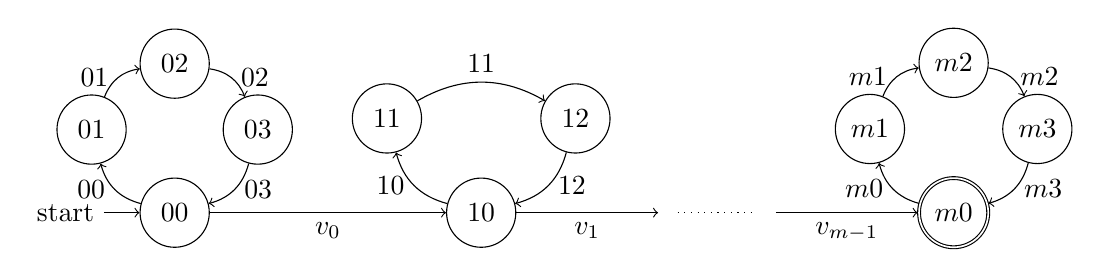
\begin{tikzpicture} 
		\node[state,initial] (q0) {$\st{0}{0}$};
		\node[state] (q1) [right = 3cm of q0] {$\st{1}{0}$};
		\node (q2) [right = 1.8cm of q1]{};
		\node (q3) [right = 1cm of q2]{};
		\node[state,accepting] (qm) [right = 1.8cm of q3] {$\st{m}{0}$};
		
		\node[state] (q01) [above left = 0.6cm of q0] {$\st{0}{1}$};
		\node[state] (q02) [above = 1cm of q0] {$\st{0}{2}$};
		\node[state] (q03) [above right = 0.6cm of q0] {$\st{0}{3}$};

		\node[state] (q11) [above left = 0.8cm of q1] {$\st{1}{1}$};
		\node[state] (q12) [above right = 0.8cm of q1] {$\st{1}{2}$};

		\node[state] (qm1) [above left = 0.6cm of qm] {$\st{m}{1}$};
		\node[state] (qm2) [above = 1cm of qm] {$\st{m}{2}$};
		\node[state] (qm3) [above right = 0.6cm of qm] {$\st{m}{3}$};

 		\draw[->] (q0) edge [bend left] node [left]{$\sym{0}{0}$} (q01) ;
 		\draw[->] (q01) edge [bend left] node [left]{$\sym{0}{1}$} (q02) ;
 		\draw[->] (q02) edge [bend left] node [right]{$\sym{0}{2}$} (q03) ;
 		\draw[->] (q03) edge [bend left] node [right]{$\sym{0}{3}$} (q0) ;
 		
 		\draw[->] (q0) edge node [below]{$v_0$} (q1) ;
 		\draw[->] (q1) edge node [below]{$v_1$} (q2) ;
 		\draw[dotted] (q2) edge (q3) ;
 		\draw[->] (q3) edge node [below]{$v_{m-1}$} (qm) ;

 		\draw[->] (qm) edge [bend left] node [left]{$\sym{m}{0}$} (qm1) ;
		\draw[->] (qm1) edge [bend left] node [left]{$\sym{m}{1}$} (qm2) ;
		\draw[->] (qm2) edge [bend left] node [right]{$\sym{m}{2}$} (qm3) ;
		\draw[->] (qm3) edge [bend left] node [right]{$\sym{m}{3}$} (qm) ;

 		\draw[->] (q1) edge [bend left] node [left]{$\sym{1}{0}$} (q11) ;
		\draw[->] (q11) edge [bend left] node [above]{$\sym{1}{1}$} (q12) ;
		\draw[->] (q12) edge [bend left] node [right]{$\sym{1}{2}$} (q1) ;
	\end{tikzpicture} }

	\caption{An example of a parametric flat automaton}
	\label{fig:sfa_def}
\end{figure}


The second step of our decision procedure is only enabled if the over-approximation is SAT. In this case, our decision procedure restricts the domain of each string variable to strings that obey some predefined and parameterized pattern.  Adjusting the parameters enlarges or prunes the potential solution space. In this paper, we propose to use patterns defined by \emph{parametric flat automata} (PFA). A PFA is a {\em flat} finite state automaton consisting of a predefined sequence of loops, each of fixed length (see Figure \ref{fig:sfa_def}). The approach based on PFA is very flexible yet allows very efficient manipulation. One can pick PFA of \emph{arbitrary structure} for search space restriction and reduce the string constraint solving problem to a linear formula satisfiability problem in polynomial-time. Furthermore, we associate a unique natural number with each character. This allows us to assume that the input alphabet is a subset of natural numbers to avoid the \textit{alphabet explosion problem} from which the approach in~\cite{abdulla2017flatten} suffers.  We label each transition between two states of a PFA with a unique \emph{character} variable (whose domain is the set of natural numbers) instead of having a transition between each two states for each symbol in the alphabet.  
Such reduction based on PFA is the key to handling string-number conversion efficiently. When we restrict the solution space to those defined by PFAs, the original undecidable problem (i.e., string constraint with string-number conversion) is reduced to the satisfiability problem of linear formulas and can be solved efficiently. 

%The battle field is in fact those SAT instances, for which we develop solutions using under-approximation. For under-approximation, we restrict the search space of each string variable to strings that obey some predefined and parameterized pattern. By adjusting the parameters, one can easily enlarge or prune out the potential solution space. In paper, we propose to use patterns defined by \emph{parametric flat automata} (PFA) (will be defined formally in Section~\ref{section:sfa}). The approach based on PFA is very flexible yet allows very efficiently manipulation. One can pick PFA of \emph{arbitrary structure} for the search space restriction and reduce the string constraint solving problem to a linear formula satisfiability problem in polynomial-time. Moreover, it avoids the \textit{alphabet explosion problem} that the approach in~\cite{abdulla2017flatten} suffers. 
%%In contrast to under-approximation based on bit-blasting~\cite{kiezun2009hampi} (i.e., limit the length of the strings and encode the string constraint to a Boolean formula), our linear formula for under-approximation still encodes possibility an infinite number of models. 
%Such reduction based on PFA is the key to handle string-number conversion efficiently. When we restrict the solution space to those defined by PFAs, the original undecidable problem (i.e., string constraint with string-number conversion) is reduced to linear formulas and can be solved efficiently. We can step-wisely enrich the PFAs and hence solve the satisfiability problem of string constraints in a systematic manner.


\begin{figure}
	\tikzset{state/.style={circle,draw=blue!50,fill=blue!20,
			thick,inner sep=0pt,minimum size=6mm}, initial text=$ $}
	
	\begin{minipage}[t]{0.1\textwidth} 
			\scalebox{0.7}{
		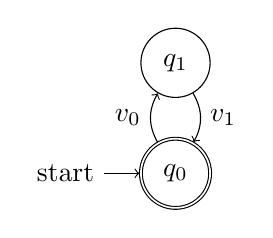
\begin{tikzpicture}
		\node[state,initial,accepting] (q0) {$q_0$};
		
		\node[state] (q01) [above = 0.5cm of q0] {$q_1$};
		
		\draw[->] (q0) edge [bend left] node [left]{$v_0$} (q01) ;
		\draw[->] (q01) edge [bend left] node [right]{$v_1$} (q0) ;
		\end{tikzpicture} }
		
		\centering
		(a) $A_x$
	\end{minipage}
	\begin{minipage}[t]{0.1\textwidth} 
			\scalebox{0.7}{
		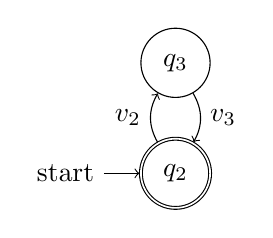
\begin{tikzpicture} 
		\node[state,initial,accepting] (q0) {$q_2$};
		
		\node[state] (q01) [above = 0.5cm of q0] {$q_3$};
		
		\draw[->] (q0) edge [bend left] node [left]{$v_2$} (q01) ;
		\draw[->] (q01) edge [bend left] node [right]{$v_3$} (q0) ;
		\end{tikzpicture} }
		
		\centering
		(b) $A_y$
	\end{minipage}
	\begin{minipage}[t]{0.2\textwidth}
			\scalebox{0.7}{
		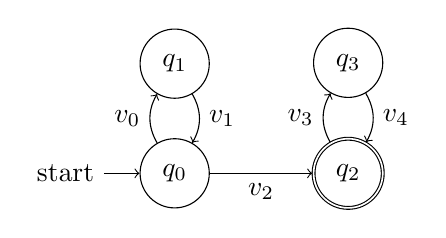
\begin{tikzpicture} 
		\node[state,initial] (q0) {$q_0$};
		\node[state,accepting] (q1) [right = 1.3cm of q0] {$q_2$};
		
		\node[state] (q01) [above = 0.5cm of q0] {$q_1$};
		
		\draw[->] (q0) edge [bend left] node [left]{$v_0$} (q01) ;
		\draw[->] (q01) edge [bend left] node [right]{$v_1$} (q0) ;
		
		\node[state] (q11) [above = 0.5cm of q1] {$q_3$};
		
		\draw[->] (q1) edge [bend left] node [left]{$v_3$} (q11) ;
		\draw[->] (q11) edge [bend left] node [right]{$v_4$} (q1) ;
		\draw[->] (q0) edge node [below]{$v_2$} (q1) ;
		\end{tikzpicture}}
		
		\centering
		(c) $A'_{x}$
	\end{minipage}
	
	\caption{Parametric flat automata of $x$ and $y$}
	\label{fig:sfa}
\end{figure}


In the following, we explain the construction of the linear formula using $\Phi$ as an example. Assume that we project the domains of $x$ and $y$ to the PFA in Figure~\ref{fig:sfa} (a) and (b), respectively. The variables $v_1$, $v_2$, $v_3$, $v_4$ in the figure are \emph{character} variables. Thus, $v_1$, $v_2$, $v_3$, $v_4$ are also integer variables. For example, from the formula $ y \in (12)^+$, we may derive $v_3=1$ and $v_4=2$. 

The linear formula produced after the domain restriction will be over variables $v_1$, $v_2$, $v_3$, $v_4$, as well as the number of occurrences of each character variable $\#v_1$, $\#v_2$, $\#v_3$, $\#v_4$. Each model of the linear formula encodes a model of the string constraint. For example, $x=``12''$ and $y=``1212''$ is encoded by the assignment $(v_1,v_2,v_3,v_4,\#v_1,\#v_2,\#v_3,\#v_4)= (1,2,1,2,1,1,2,2)$. The assignment says, for example, that $x$ is the parametric word obtained by traversing the loop of $A_x$ once (because $\#v_1 = \#v_2 = 1$), which is $v_1v_2$. Under the assignment $v_1=1$ and $v_2=2$, we obtain $x=``12''$.

If a model of the produced linear formula is found, then the procedure concludes SAT with an assignment to the string variables. If not, our procedure changes the PFAs to be more expressive ones (by adding more states and transitions) to systematically search for a solution. Depending on the implementation, one may choose to report unknown after some certain steps.




%For over-approximation, there are a few existing algorithms~\cite{parosh2019chain,z3,chen2019decision}, our framework does not set any restriction on which algorithm to be used. In our experiences, the UNSAT instances in all available benchmarks are not that difficult, and the differences between the major algorithms are very small. In our tool \tool, we use a version that is a simple adaption of the algorithm in~\cite{parosh2019chain}.

%The battle field is in fact those SAT instances, for which we develop solutions using under-approximation. For under-approximation, we restrict the search space of each string variable to strings that obey some predefined and parameterized pattern. By adjusting the parameters, one can easily enlarge or prune out the potential solution space. In paper, we propose to use patterns defined by \emph{parametric flat automata} (PFA) (will be defined formally in Section~\ref{section:sfa}). The approach based on PFA is very flexible yet allows very efficiently manipulation. One can pick PFA of \emph{arbitrary structure} for the search space restriction and reduce the string constraint solving problem to a linear formula satisfiability problem in polynomial-time. Moreover, it avoids the \textit{alphabet explosion problem} that the approach in~\cite{abdulla2017flatten} suffers. 
%%In contrast to under-approximation based on bit-blasting~\cite{kiezun2009hampi} (i.e., limit the length of the strings and encode the string constraint to a Boolean formula), our linear formula for under-approximation still encodes possibility an infinite number of models. 
%Such reduction based on PFA is the key to handle string-number conversion efficiently. When we restrict the solution space to those defined by PFAs, the original undecidable problem (i.e., string constraint with string-number conversion) is reduced to linear formulas and can be solved efficiently. We can step-wisely enrich the PFAs and hence solve the satisfiability problem of string constraints in a systematic manner.

\hide{More concretely, based on the PFA encoding, we manage to translate the string constraint with string-number function to an equisatisfiable pure numerical constraints. Thus the problem is significantly simplified. We show that if we restrict the variable to arbitrary PFA, one can convert the a string constraint with string-number function to an integer constraint consisting of both polynomials and exponentials. Solving such kind of constraints is a very difficult task. For simpler cases where the variables are real numbers, decision procedures for different subclass polynomial-exponential equations exists~\cite{gan2015decidability,kincaid2019closed,achatz2008deciding}. To the best of our knowledge, the satisfiability problem of polynomial-exponential equations is still open. For efficiency reason, we propose to use PFA with specific structural constraint to handle string-number conversion function. That is, if we encountered a constraint $y=\sti{x}$, then we always restrict the domain of $x$ to some specific kind of PFA, instead of allowing arbitrary PFAs. This allows us to convert a string constraint with string-number conversion function to an equisatisfiable linear formula, which can be solved very efficiently. }

\hide{Our string constraint solving procedure can be easily integrated in a \emph{satisfiability module theory (SMT)} solver as a theory solver. The integration allows us to express string operations that cannot be reduced to the type of constraints (regular, equality, integer, string-number conversion) supported by our procedure. For example, we can encode \texttt{split} using the code fragment in Figure~\ref{fig:smt_string}. Other functions such as \texttt{replaceAll} and \texttt{reverse} can be encoded in a similar manner. The performance of such encoding might not be as good as those that provide direct support to those operations, but at least it works for some cases in our experiments. Further details of the combination as well as some other implementation details can be found in Section~\ref{section:implementation}.



\begin{figure}
	\begin{Verbatim}[fontsize=\scriptsize,xleftmargin=-4cm]
				(define-fun-rec split ((x String)(y String)(xIdx Int)(aIdx Int)) 
				(Array Int String)
				(ite (= xIdx (str.len x))
				 (store ((as const (Array Int String)) "") aIdx x)
				 (ite (= y (str.at x xIdx)) 
				  (store 
				   (split (str.substr x (+ xIdx 1) (- (str.len x) 1) ) 
				   0 (+ aIdx 1) y) 
				   aIdx
				   (str.substr str 0 xIdx)
				  )
				  (split x (+ xIdx 1) aIdx y)
				 )
				)
			\end{Verbatim}
	 	 				
	 	\caption{Encoding \texttt{Split(x,y)} to an SMTLIB2 formula using recursive functions and the array theory. The recursive function \texttt{split (x y 0 0)} returns an array of type \texttt{(Array Int String)} that maps an index $i$ to the $i$th component (separated by the character $y$ ) of $x$.}
	 	\label{fig:smt_string}
\end{figure}

}


To demonstrate the usefulness of our approach, we have implemented our decision procedure in an open source solver, called {\tool} and evaluated it on a large set of benchmarks obtained from literatures and from symbolic execution of real world programs. The experimental results show that {\tool} is among the best tools for solving basic string constraints and significantly outperforms all other tools on benchmarks with string-number conversion constraints. In this benchmark, the total amount of tests cannot be solved by {\tool} is only a half to the second best tool.


\smallskip

\noindent
{\bf Summary of the Contributions}

\begin{itemize}

\item An {\em efficient} procedure for checking satisfiability
of string constraints with string-number conversion constraints.



\item The introduction of the class of \emph{parametric flat automata} which uses character variables as transition labels instead of characters. This allows us to avoid the {alphabet explosion problem} that the approach in~\cite{abdulla2017flatten} when it comes to handle string-number conversion constraints.


\item An algorithm that translates the satisfiability string constraints to the satisfiability of a linear formula  in polynomial-time when  the search space restricted by PFAs.


\item An open source tool with experimental
results that demonstrate the efficiency of
our approach on both existing and real-life benchmarks
\end{itemize}


\hide{
To ease presentation, in the paper, we only consider string constraints consisting of \emph{equality constraints (a.k.a. word equation)}, \emph{regular constraints}, \emph{length constraints}, and \emph{string-number conversion} functions. 	
	
suggest restricting the string domain to $0^*[0-9]^k$, where $k$ is the maximum 
digit allowed in the corresponding number value. In programming languages 
such as JavaScript or Python, a number with $k$ digits can be converted from a 
string of length arbitrarily longer than $k$. For example, $12 = 
str2int(``0000012")$. That is why we use $0^*$ at the beginning of the pattern.
Under this domain, we can convert the string-number conversion constraints to 
linear integer constraints, which is much easier to solve. In our experience, 
usually, it suffices to find a solution using a small $k$ for a satisfiable 
constraint. Note that a 64-bit integer number corresponds to a word with 
$k\leq 21$.

Given a formula that is a boolean combination of different types of string constraints, e.g., $\phi=(|x| = |y| \vee \sti{x} = \sti{y})\wedge x = y$, an SMT solver based on the DPLL(T) algorithm~\cite{} treats each string constraint $|x| = |y|$, $\sti{x} = \sti{y}$, $xy=yx$ as a boolean variable, and systematically guesses possible solutions without considering their semantics as string constraints. E.g., the solver may guess $\neg(|x| = |y|)$, $(\sti{x} = \sti{y})$, and $(x =y)$. This is a valid guess if all the string constraints are just interpreted as boolean variables, but invalid when their semantics as string constraints are considered, because it cannot be the case that $x$ and $y$ are the same string $(x =y)$, but they are of different lengths $( \neg (|x| = |y|))$.


The approach combines techniques from both automata theory and SMT solving to explore the model space of a string constraint systematically. More specifically, an SMT solver based on the DPLL(T) algorithm~\cite{} is used to convert the satisfiability of a string constraint, which is an arbitrary boolean combination of string predicates, to the satisfiability problem of a set of string constraints in the form of conjunctions of string predicates.




}

%%%%%%%%%%%%%%%%%%%%%%%%%%%%%%%%%%%%%%%%%%%%%%%%%%%%%%%%%%%%%%%%%%%%%%%%%%%%%%%
%\section{Overview} \label{section:overview}
%%%%%%%%%%%%%%%%%%%%%%%%%%%%%%%%%%%%%%%%%%%%%%%%%%%%%%%%%%%%%%%%%%%%%%%%%%%%%%%
%
%Here we try to explain the approach using a toy example $\Phi = \{xy=yx, n = \sti{x}, n >3 ,|y|>|x|, y \in (12)^+\}$. Notice that $\Phi$ is satisfiable. E.g., it has a model $x=``12''$ and $y=``1212''$.
%
%For proving UNSAT, our framework does not set any restriction on which decision procedure to use. One can select any decision procedure they want to use and ``over-approximate'' the input constraint to one that falls in the decidable fragment, e.g., the acyclic fragment~\cite{abdulla2014string}, the straight-line fragment~\cite{chen2019decision}, or the chain-free fragment~\cite{abdulla2019chain}. For instance, we can convert $xy=yx$ to two formulas $\{x_1=xy, x_2=yx\}$ using two auxiliary variables $x_1,x_2$ and replace the constraint $n=\sti{x}$ with $n=-1 \vee (n\neq -1 \wedge x\in [0-9]^*$). This produce new formulas that over-approximate the original ones and fall in the chain-free fragment~\cite{abdulla2019chain}, which is decidable. Since $\Phi$ is satisfiable, the over-approximation module will not return UNSAT. In our implementation \tool, we further add heuristics trying to derive the constant value of any side of the constraint $n=\sti{x}$ to refine the over-approximation. For instance, assume in some other cases, we can derive the value of $n=12$ from some integer constraints. In such case, we can further derive the value of $x$ is in the regular language $(0^*12)$. 
%
%Then our procedure will restrict the domain of each string variables to the language defined by some parametric flat automata (PFA) and convert them to equisatisfiable linear formula. The details of the under-approximation component will be described in Section~\ref{section:under_approximate}. Here we try to explain what the linear formula looks like by an example. Assume that we project the domain of $x$ and $y$ to the PFA in Figure~\ref{fig:sfa} (a) and (b), respectively. The variables $v_1$, $v_2$, $v_3$, $v_4$ in the figure are \emph{character} variables. One special treatment we do in this paper is that we encoding characters as natural numbers. So $v_1$, $v_2$, $v_3$, $v_4$ are also integer variables. For example, from the formula $ y \in (12)^+$, we may derive $v_3=1$ and $v_4=2$. 
%
%The linear formula produced after the domain restriction will be over variables $v_1$, $v_2$, $v_3$, $v_4$, as well as, the number of occurrences of each character variables $\#v_1$, $\#v_2$, $\#v_3$, $\#v_4$. Each model of the linear formula encodes a model of the string constraint. For example, $x=``12''$ and $y=``1212''$ is encoded by the assignment $(v_1,v_2,v_3,v_4,\#v_1,\#v_2,\#v_3,\#v_4)= (1,2,1,2,1,1,2,2)$. The assignment says, for example, that $x$ is the parametric word obtained by traversing the loop of $A_x$ once (because $\#v_1 = \#v_2 = 1$), which is $v_1v_2$. Under the assignment $v_1=1$ and $v_2=2$, we obtain $x=``12''$.
%
%If a model of the produced linear formula is found, then the procedure concludes SAT with an assignment to the string variables. If not, our procedure step-wisely change the PFA to more expressive ones (by adding more states and transitions) to systematically search for the solution. Depending on the implementation, one may choose to report unknown after some certain steps.
%


%%%%%%%%%%%%%%%%%%%%%%%%%%%%%%%%%%%%%%%%%%%%%%%%%%%%%%%%%%%%%%%%%%%%%%%%%%%%%%
\section{Preliminaries} \label{section:preliminary}
%%%%%%%%%%%%%%%%%%%%%%%%%%%%%%%%%%%%%%%%%%%%%%%%%%%%%%%%%%%%%%%%%%%%%%%%%%%%%%
%We use $\mathbb{N}$ and $\mathbb{Z}$ to denote the sets of natural numbers and 
%integers. For a set $A$, we use $|A|$ to denote its size. For a string $w$, we 
%use $|w|$ to denote its length and $|w|_a$ to denote the number of occurrences of $a$ in $w$. We $\epsilon$ to denote an empty string and use $w_1\cdot w_2$ to denote the concatenation of strings $w_1$ and $w_2$. Let $S$ be a finite set of symbols. We use $S^+$ to denote the set of string over $S$ and $S^* = S^+\cup \{\epsilon\}$. We define $S_\epsilon =S\cup\{\epsilon\}$. A language 
%$L$ over $S$ is a set of strings in $S^*$. 
%
%A \emph{finite automaton} is a tuple $(Q,T,\Sigma,q_0,q_m)$, where $Q$ is the set of states, $T\subseteq Q\times (\Sigma\cup \{\epsilon\} )\times Q $ is the set of transition relation, $\Sigma$ is the alphabet, $q_0$ is the initial state, and $q_m$ is the final state. The semantics of finite automaton is defined in the standard manner. We use $L(A)$ to denote the regular language, i.e., set of accepted strings, of the automaton $A$.

%Given a finite automaton $A$ over $\{a_1,a_2,\ldots,a_n\}$, the Parikh image of $L$ is the set $\{(|w|_{a_1},\ldots, |w|_{a_n}) \mid w \in L(A) \}$, i.e., the number of occurrences of each symbol $\{a_1,a_2,\ldots,a_n\}$ of words in $L(A)$. Moreover, one can construct from $A$ in linear time a Presburger formula $\phi_A(v_1, \ldots,v_n)$ such that $\phi(c_1, \ldots,c_n) \iff (c_1, \ldots,c_n)$ in the Parikh image of $L$~\cite{SeidlSMH04}.

We use $\mathbb{N}$ and $\mathbb{Z}$ to denote the sets of natural numbers (including 0) and 
integers. For a set $A$, we use $|A|$ to denote its size. 
For $n,m\in\nat$, we write $[n,m]$ for the set of natural numbers 
%(or symbols in $\Sigma$) 
$\{k\mid n\leq k \leq m\}$. 
The function $f$ with the domain restricted to $D$ is denoted by $\restrict f D$,
and a set of functions $F$ restricted to $D$ is $\restrict F D = \{\restrict f D \mid f \in F\}$.
An \emph{alphabet} is a finite set $\Sigma$ of \emph{characters} and a \emph{word} over $\Sigma$ is a sequence $w = a_1\ldots a_n$ of characters from $\Sigma$, with $\epsilon$ denoting the \emph{empty word}. 
We use $w_1\cdot w_2$ to denote the \emph{concatenation} of words $w_1$ and $w_2$.
$\Sigma^*$ is the set of all words over $\Sigma$, $\Sigma^+ = \Sigma^*\setminus \{\epsilon\}$, $\Sigma_\epsilon = \Sigma\cup\{\epsilon\}$, and 
A \emph{language} over $\Sigma$ is a subset $L$ of $\Sigma^*$. 
%
We use $|w|$ to denote the length of $w$ and $|w|_a$ to denote the number of occurrences of the character $a\in \Sigma$ in $w$. 

A \emph{finite automaton} (FA) is a tuple $(Q,T,\Sigma,q_i,q_f)$, where $Q$ is the set of \emph{states}, $T\subseteq Q\times \Sigma \times Q $ is the set of \emph{transitions}, $\Sigma$ is the alphabet, $q_i$ is the \emph{initial state}, and $q_f$ is the \emph{final state}. 
%The semantics of finite automaton is defined in the standard manner. 
A \emph{run} of $A$ over a word $w = a_1\cdots a_n$ is a sequence of transition $(q_0,a_1,q_1),(q_1,a_1,q_2),\ldots,(q_{n-1},a_n,q_n)$. The run is \emph{accepting} if $q_0 = q_i$ and $q_i = q_f$ and $w$ then is \emph{accepted}.
The \emph{language} of $A$ is the set $L(A)$ of all accepted words.

%Through the paper, we will use quantifier-free linear integer arithmetic formulas, and call them \emph{linear formulas} for short.  
%Given a linear formula $\phi$, a set of variables $V$, and an \emph{interpretation} of $V$, i.e., a function $I:V\rightarrow \nat$, 
%we denote by $I\models_V \phi$ that $I$ satisfies $\phi$ (which is defined in the standard manner), and call $I$ a \emph{model} of $\phi$ over $V$. 
%
%\lh{Our use of indexing by $V$ in the text later is not very nice. Add this for clarity?: If $V$ contain additional variables not present in $\phi$, the these might be assigned arbitrary values by $I$. If $V$ is missing some of the variables of $\phi$, then it must be possible to complete $I$ with assignment of the missing variables into a satisfying assignment of $\phi$ (as in existential quantification).}
%We use $\modelsof \phi$ to denote the set all models of $\phi$ over $V$. 
%We drop the reference to $V$ and write just ``model of $\phi$'', $\modelsof \phi$, and $\models$ when no confusion may arise. For a set of interpretations $S$, we use $S_\Sigma$ to denote the set of interpretations obtained from $S$ by projecting the domain to $\Sigma$.

Through the paper, we will use quantifier-free linear integer arithmetic formulas, and call them \emph{linear formulas} for short.  
Given a linear formula $\phi$ over variables $V$ and an \emph{integer interpretation} of $V$, a function $I:V\rightarrow \integers$, 
we denote by $I\models \phi$ that $I$ satisfies $\phi$ (which is defined in the standard manner), and call $I$ a \emph{model} of $\phi$. 
We use $\modelsof \phi$ to denote the set all models of $\phi$. 
%
%Let $J$ and $J'$ be two sets integer interpretations, $J$ containting interpretation of variables $V$ and $J'$ of variables $V'$. 
%We say that $J$ and $J'$ are \emph{equivalent}, written $J\iequiv J'$, if their interpretations restricted to the common variables are the same, that is, if 
%$\{\restrict I {V\cap V'} \mid I \in J\} = \{\restrict {I'} {V\cap V'} \mid I' \in J'\}$. We may write $J\eqwrt{V\cap V'} J'$ if we wish to made the common variables explicit.


The \emph{Parikh image} of a word $w\in \Sigma^*$ is the assignment 
$\parikhof w$ that for every character $a\in\Sigma$ maps the \emph{Parikh variable} $\#a$ to the number of occurrences of $a$ in $w$.
Formally, let $\pvarsof S$ denote the set of Parikh variables $\{\#s \mid s\in S\}$ obtained from a set $S$. 
The Parikh image of $w$ is a function $\parikhof w:\pvarsof \Sigma \rightarrow \nat$ such that $\parikhof w (\#a) = |w|_a$. 
The Parikh image of a language $L$ is the set of Parikh images $\parikhof L = \{\parikhof w \mid w \in L\}$. %and the Parikh image of an FA $A$ is Parikh image of its language, $\parikhof{A} = \parikhof{L(A)}$. 
%
It is well known that $\parikhof {L(A)}$ can be efficiently computed in the form of linear formula:



\begin{lemma}[\cite{SeidlSMH04}]
$\parikhof{L(A)}$ of an FA $A$ can be computed in the form of a linear formula $\parikhfof{A}$ such that 
%$\modelsof{\parikhfof A}_{\#\Sigma} = \parikhof{L(A)}$, 
$\modelsof{\parikhfof A} = \parikhof{L(A)}$, 
in time linear to the size of $A$.
\end{lemma}



 


%%%%%%%%%%%%%%%%%%%%%%%%%%%%%%%%%%%%%%%%%%%%%%%%%%%%%%%%%%%%%%%%%%%%%%%%%%%%%%
\section{String Constraints} \label{section:sc}
%%%%%%%%%%%%%%%%%%%%%%%%%%%%%%%%%%%%%%%%%%%%%%%%%%%%%%%%%%%%%%%%%%%%%%%%%%%%%%


In this section, we formally define string constraints. To begin with, we fix an finite alphabet $\Sigma \subseteq \mathbb{N}$. Note that here we assume the alphabet is a finite subset of natural numbers. Essentially, we try to capture the numerical encoding of the corresponding symbols in computers (e.g., in ASCII, `A' is encoded as $65$). We assume there is an one-one mapping between numbers in $\Sigma$ and the character it encodes. For the simplicity of presentation, we assume the character `$0$' is mapped to the number $0$, `$1$' to $1$,$\ldots$, and `$9$' to $9$. For other character $c$, we use $\enc{c}$ to denote the number that it maps to. Notice that this approach is general enough to support any finite set of characters. 


We call $\vars$ the set of \emph{string variables} ranging over $\Sigma^*$ and $\varn$ the set of \emph{integer variables} ranging over $\mathbb{Z}$.
For a variable $x$, we call its primed version (e.g., $x'$) or indexed versions (e.g., $x_1$) its \emph{variants}.
In this paper, we use $x,y$ (or their variants) to denote string variables and $n$ (or its variants) to denote integer variables.

An \emph{interpretation over $\vars$ and $\varn$} is a mapping $I$ from $\vars\cup \varn$ to $\Sigma^* \cup \mathbb{N}$. A \emph{term} is an element in $(\vars\cup \Sigma)^*$. We lift the interpretation $I$ to terms and linear constraints in the standard manner. 

We will use four types of \emph{atomic string constraint}: 

An \emph{equality constraint} $\phi_e$ is of the form $t_1 = t_2$ where $t_1, 
t_2$ are terms in $(\vars\cup \Sigma)^*$. The \emph{model} of $\phi_e$ is the set of interpretations $\modelsof{\phi_e}=\{I\mid 
I(t_1)=I(t_2)\}$. A \emph{disequality constraint} $\phi_d$ is of the form $t_1 \neq 
t_2$ and is interpreted analogously.

An \emph{integer constraint} $\phi_i$ is a linear constraint over the variables in $\varn$ and length of a word $|x|$ for all $x \in \vars$.
%Formally, assume that $\vars=\{x_i,\ldots,x_n\}$ and $\varn=\{y_i,\ldots,y_m\}$, a length constraint is of the form $(\sum_{i\in[1,n]}(j_i \times \sti{x_i}+k_i\times |x_i|)+ \sum_{i\in[1,m]}(l_i \times y_i)) \odot k$, where $\odot \in \{>,\geq, =, \leq, <\}$, and $j_i,k_i,l_i,k\in \mathbb{Z}$. We define $\modelsof{\phi}= \{I \mid (\sum_{i\in[1,n]}(j_i \times \sti{I(x_i)}+k_i\times |I(x_i)|)+ \sum_{i\in[1,m]}(l_i \times I(y_i))) \odot k \}$.
We define $\modelsof{\phi_i}= \{I \mid I(\phi_i)= \true \}$. 
\lh{should we somehow define the sematntics of the lengt constraints more precisely? That is, how is the value of $|x|$ related to the value of $x$. ?}

A \emph{regular constraint} $\phi_r$ is of the form $x \in L(A)$ where $x$ is a string variable and $A$ is a finite automaton. The \emph{model} of $\phi_m$ is the set of interpretations $\modelsof{\phi_m}=\{I\mid 
I(x) \in L(A) \}$. 

A \emph{string-number conversion constraint} $\phi_s$ is of the form $n=\sti{x}$, where the function $\sti{x}$ is defined as follows. For $a\in [0,9]$, we have $\sti{a}=a$ and for $s \cdot a \in [0,9]^+$, $\sti{s\cdot a} = 10\times \sti{s}+a$. For $s\notin [0,9]^+$, $\sti{s}=-1$. We define $\modelsof{\phi_s}= \{I \mid I(n)= \sti{I(x)} \}$. The \emph{number-string} conversion constraint $x=\its{n}$ is treated as a syntactic sugar for $n=\sti{x}$.

A \emph{string constraint} is then a conjunction of atomic string constraints, with the semantics defined in the standard manner. It is \emph{satisfiable} if its semantics is nonempty.

Notice that only positive integer is supported in the string-number conversion function. This is the semantics used by most of the SMT solvers, and hence we follow it in this paper. The encoding has a benefit that it can also handle the case where $x$ is ``not a number'', using the condition $\sti{x} = -1$.

Supporting only positive integer is not a strong restriction, since conversing from negative integer can still be encoded using the positive only version. More specifically, if we want to say $n \in \varn$ is the integer value of the string $x \in \Sigma^*$, we can write the following constraint (ignore the case that $x$ is ``not a number'', which can also be encoded using more conditions):
$$(n= \sti{x}) \vee (n=-\sti{x'} \wedge x = \enc{-}\cdot x')$$
Recall that $\enc{-}$ is the integer encoding of the minus symbol `$-$'. The \emph{number-string conversion function} $\its{n}$ is defined symmetrically. We have $x = \its{n}$ iff $y= \sti{n}$. 


%\section{Under-approximation} \label{section:under_approximate}
%In this section, we describe formally how to restrict the domain of string variables to patterns defined by \emph{parametric flat automata} (PFA) (Section~\ref{section:sfa}) and hence convert string constraints $\insc$ to a set of equisatisfiable linear formulas $\outlf$ in polynomial-time. We assume all disequality constraint $t_1 \neq t2$ are already converted to equal-satisfiable equality constraints and integer constraints in the standard way~\cite{abdulla2015norn}. 
%
%We pick a PFA for each variable in $\vars$ at the beginning of the decision procedure and then construct the set of linear integer constraints in a stepwise manner. In each step, we take a string constraint from $\insc$ and depending on the type of the string constraint, we execute the corresponding procedure to produce the linear integer constraints and add them to the output linear formulas $\outlf$. We also add constraints to $\outlf$ to ensure all character variables of the PFAs only pick values from $\Sigma_\epsilon$.
%
%More concretely, at the beginning, we move all integer constraints in $\insc$ to the output linear formulas $\outlf$. After this step, $\insc$ is the union of the three sets of constraints: the equality constraints, the regular constraints, and the string-number conversion constraints. For all string variables $x$ that occurs in a string-number conversion constraint $n= \sti{x}$, we follow the rule that will be described in Section~\ref{section:s2i} to pick the corresponding PFA. We do not set any restriction to the selection of PFA for other string variables. The selection is an implementation decision. We will describe the PFA selection strategy of \tool in Section~\ref{section:implementation}. 
%
%After the PFA for each variable is selected, we step-wisely pick and remove a string constraint from $\insc$, executing the corresponding procedure to create equisatisfiable linear constraints, and add all the results to $\outlf$. The procedures for regular, equality and string-number conversion constraints are in Sections~\ref{section:mem},~\ref{section:eq}, and~\ref{section:s2i}, respectively. In the rest of the section, we assume each string variable $x$ is restricted to a PFA $A_x$ with the set of character variables~$V_x$.
%
%
% 
%
%
%
%\hide{We replace it with the following constraints.
%	
%	$$
%	\begin{array}{c}
%	(|x_1|+ |x_2|+ \cdots +|x_n| \neq |x_{n+1}| + |x_{n+2}|+ \cdots +|x_m|)\vee \\
%	\left(
%	\begin{array}{cccc}
%	
%	y_1\cdot y_2\cdot y_3 &=& x_1\cdot x_2 \cdots x_n &\wedge\\
%	y_1 \cdot y'_2 \cdot y'_3 &=& x_{n+1}\cdot x_{n+2} \cdots x_m &\wedge\\
%	|y_2|&=&|y'_2|=1
%	\end{array}
%	
%	\right)
%	\end{array}
%	$$
%	
%	The second disjunct says that the constraints $x_1\cdot x_2 \cdots x_n$ and $x_{n+1}\cdot x_{n+2} \cdots x_m$ have a common prefix $y_1$, but the next character $y_2$ and $y'_2$ is different. In an more efficient implementation, one just project $y_2$ and $y'_2$ to a PFA that accept only symbolic words $v_1$ and $v'_1$, respectively (the PFA has no loop and only one transition). }
%
%
%\yfc{say handling regular constraint can be exponential to the number of constraints, but in our under-approximation, it is polynomial.}





%%%%%%%%%%%%%%%%%%%%%%%%%%%%%%%%%%%%%%%%%%%%%%%%%%%%%%%%%%%%%%%%%%%%%%%%%%%%%%
\section{Parametric Flat Automata} \label{section:sfa}
%%%%%%%%%%%%%%%%%%%%%%%%%%%%%%%%%%%%%%%%%%%%%%%%%%%%%%%%%%%%%%%%%%%%%%%%%%%%%%

We introduce \emph{parametric flat automata} that will be used to define patterns 
used by the under-approximation module to restrict the domain of string variables. 

\paragraph{Flat automata}
First, we say that an FA 
$A = (Q,T,\Sigma,\st{0}{0},\st{m}{0})$ is \emph{flat} if it satisfies the following structural constraints:
\begin{enumerate}
	\item The final state $\st{m}{0}$ is reached from  the initial state $\st{0}{0}$ through a straight path of $m-1$ transitions $(\st{i}{0},a_i,\st{i+1}{0}) \in T$, $\st{i}{0} \in Q$ for $i\in[0,m-1]$. 
	\item  
Each state $\st{i}{0}$ is the origin of a unique simple cycle of the length $l_i\in\mathbb{N}$, consisting of states $\st{i}{j-1} \in Q$ and transitions $(\st{i}{j-1}, a_{i}^{j-1}, \st{i}{j \bmod l_i})$ for $j\in [1,l_i]$. 
Notice that the case when $l_i = 0$ is also admissible and means that there is no cycle on $q_i$.
	\item Each character in $\Sigma$ appears on at most one transition. 
\end{enumerate} 

The crucial feature of flat automata is that their semantics can be faithfully represented by a linear formula and handled efficiently by an SMT solver. 
\lh{, allowing to circumvent more costly automata algorithms and decision procedures. Concretize and justify this better?}
%
This is facilitated by flatness, which guarantees that 
every parametric word $w\in L(A)$ is uniquely determined by its Parikh image $\parikhof{w}$. 
In fact, the Parikh image of a word $w\in L(A)$ can be seen as an encoding of $w$ and can be uniquelly decoded:


\begin{lemma}\label{lemma:decoding}
For an flat FA $A$, there is a function $\decode A$ such that for each $w\in L(A)$, $\decode A(\parikhof w) = w$. 
\end{lemma}
%
\begin{proof}
Indeed, since every variable appears on at most one transition, then the $\parikhof w$ value of all variables appearing within the same cycle of $A$ is the same, and it is equal to the number of repetitions of that cycle in the accepting run. 
%
The accepting run on $w$ (and so $w$ itself) can thus be reconstructed from $\parikhof w$. 

More concretely, the function $\decode A$ can be implemented as follows. 
Given $\pim:\#\cvar\rightarrow\nat$,
and assuming that the lengths of the loops of $A$ are $l_0,\ldots,l_{m-1}$, 
$\decode A(\pim)$ is constructed as the word $w_0 a_{0} \ldots a_{m-1} w_{m-1}$ where for each $i\in [0,m-1]$,
$w_i = (a_i^0 \cdots a_i^{l_{i-1}})^{\pvarsof {a_i^0}}$ if $l_i >0$ and $w_i = \epsilon$ if $l_i = 0$. 
\end{proof}
%
For example, in the automaton of Figure~\ref{fig:sfa_def}, 
from $\parikhwof x {v_0} = \parikhwof x {v_1} = \cdots = \parikhwof x {v_{m-1}}=1$ and $\parikhwof x {v^0_1}=\parikhwof x {v^1_1}=\parikhwof x {v^2_1}=2$ we derive that $x=v_0(v^0_1v^1_1v^2_1)^2v_1\cdots v_{m-1}$. 

\paragraph{Parametric (flat) automata}
Next we define \emph{parametric automaton} (PA) as a pair  $\pa = (A,\paf)$ where 
$A$ is an automaton operating over an alphabet $\cvar$ of \emph{character variables}  
and $\paf$ is an \emph{interpretation constraint}, a linear formula over $\cvar$. 
\emph{Parametric flat automaton (PFA)} is then a parametric automaton with its finite automaton flat.

Parametric automata accept words over $\cvar$, called \emph{parametric words}, but we still use them as representations of languages over $\Sigma$. 
%
Namely, words over $\cvar$ are interpreted as words over $\Sigma$ under an
\emph{interpretation of $\cvar$},
%
a mapping $I:\cvar\rightarrow\Sigma_\epsilon$. 
For a parametric word $x= v_1v_2\cdots v_k$ over $\cvar$, its interpretation $I(x)$ is then defined as $I(v_1)\cdot I(v_2)\cdot \ldots \cdot I(v_k)$.
%
We define the semantics of $x$ as the set $\semof x$ of all possible interpretations of $x$, the semantics of a language $L\subseteq V^*$ is the union $\semof L = \cup_{x\in L} \semof{x}$ of semantics of its words, and the semantics of a PA is the semantics of its language restricted by the formula $\paf$, that is,  
$\semof {\pa} = \{I(w) \mid w\in L(A),I\in\semof \paf\}$. 


Since every word $w \in \semof{\pa}$ is uniquely determined by a parametric word $x\in L(A)$ and an interpretation $I\in\semof{\paf}$ such that $w = I(x)$, and since $x$ is uniquely determined by its Parikh image, i.e.,  
$x = \decode \pa(\parikhof x)$, 
we may say that the assignment $I \cup \parikhof x$ uniting the interpretation $I:\cvar\rightarrow\Sigma_\epsilon$ and the Parikh image $\parikhof x:\#\cvar\rightarrow \nat$ \emph{$\pa$-encodes} $w$. Lemma~\ref{lemma:decoding} implies that such $\pa$-encoding can be uniquely decoded. 
We may hence extend the decoding function $\decode \pa$ to united assignments $e:\cvar\cup\#\cvar \rightarrow \nat$ 
so that $\decode \pa(I \cup \parikhof x) = w$. 
We again lift the decoding function to sets of united assignments in the standard manner.
The following corollary of Lemma~\ref{lemma:decoding} states that encodings of words in $\semof{\pa}$ are encodings of parametric words of $L(A)$ paired with arbitrary interpretations of character variables $\cvar$ that satisfy $\paf$:

\begin{corollary}\label{corollary:pfa}
For a PFA $\pa = (A,\paf)$,
\\
\centerline{$\semof {\pa} = \decode \pa \{(I\cup \pim)\mid \pim\in\parikhof{L(A)} ,I\in\semof\paf\}$.}
\end{corollary}
%

Last, we define the encoding function as a counterpart of the decoding. Given a PFA $\pa$ and a language $L\subseteq \Sigma^*$, the set of \emph{$\pa$-encodings} of the words in $L$ is defined as
$\encode \pa (L) = \{e \mid \decode \pa (e) \in L\}$. 
%
Notice that only the words from $L\cap \semof \pa$ have a $\pa$-encoding, 
hence $\encode \pa(L) = \encode \pa(L\cap\semof \pa)$, and so due to Corollary~\ref{corollary:pfa}, $\decode \pa({\encode \pa}(L)) = L\cap\semof \pa$.

%\section{Under-approximation} \label{section:under_approximate}
%In this section, we describe formally how to restrict the domain of string variables to patterns defined by \emph{parametric flat automata} (PFA) (Section~\ref{section:sfa}) and hence convert string constraints $\insc$ to a set of equisatisfiable linear formulas $\outlf$ in polynomial-time. We assume all disequality constraint $t_1 \neq t2$ are already converted to equal-satisfiable equality constraints and integer constraints in the standard way~\cite{abdulla2015norn}. 
%
%We pick a PFA for each variable in $\vars$ at the beginning of the decision procedure and then construct the set of linear integer constraints in a stepwise manner. In each step, we take a string constraint from $\insc$ and depending on the type of the string constraint, we execute the corresponding procedure to produce the linear integer constraints and add them to the output linear formulas $\outlf$. We also add constraints to $\outlf$ to ensure all character variables of the PFAs only pick values from $\Sigma_\epsilon$.
%
%More concretely, at the beginning, we move all integer constraints in $\insc$ to the output linear formulas $\outlf$. After this step, $\insc$ is the union of the three sets of constraints: the equality constraints, the regular constraints, and the string-number conversion constraints. For all string variables $x$ that occurs in a string-number conversion constraint $n= \sti{x}$, we follow the rule that will be described in Section~\ref{section:s2i} to pick the corresponding PFA. We do not set any restriction to the selection of PFA for other string variables. The selection is an implementation decision. We will describe the PFA selection strategy of \tool in Section~\ref{section:implementation}. 
%
%After the PFA for each variable is selected, we step-wisely pick and remove a string constraint from $\insc$, executing the corresponding procedure to create equisatisfiable linear constraints, and add all the results to $\outlf$. The procedures for regular, equality and string-number conversion constraints are in Sections~\ref{section:mem},~\ref{section:eq}, and~\ref{section:s2i}, respectively. In the rest of the section, we assume each string variable $x$ is restricted to a PFA $A_x$ with the set of character variables~$V_x$.
%
%
% 
%
%
%
%\hide{We replace it with the following constraints.
%	
%	$$
%	\begin{array}{c}
%	(|x_1|+ |x_2|+ \cdots +|x_n| \neq |x_{n+1}| + |x_{n+2}|+ \cdots +|x_m|)\vee \\
%	\left(
%	\begin{array}{cccc}
%	
%	y_1\cdot y_2\cdot y_3 &=& x_1\cdot x_2 \cdots x_n &\wedge\\
%	y_1 \cdot y'_2 \cdot y'_3 &=& x_{n+1}\cdot x_{n+2} \cdots x_m &\wedge\\
%	|y_2|&=&|y'_2|=1
%	\end{array}
%	
%	\right)
%	\end{array}
%	$$
%	
%	The second disjunct says that the constraints $x_1\cdot x_2 \cdots x_n$ and $x_{n+1}\cdot x_{n+2} \cdots x_m$ have a common prefix $y_1$, but the next character $y_2$ and $y'_2$ is different. In an more efficient implementation, one just project $y_2$ and $y'_2$ to a PFA that accept only symbolic words $v_1$ and $v'_1$, respectively (the PFA has no loop and only one transition). }
%
%
%\yfc{say handling regular constraint can be exponential to the number of constraints, but in our under-approximation, it is polynomial.}

\section{Flat Domain Restriction}
\label{section:under_approximate}

%
In this section, we describe formally how to restrict the domain of string variables to patterns defined by PFA. 
We start the description of the algorithm that converts a string constraint $\insc$ to a linear formula $\outlf$, called the \emph{flattening} of $\insc$, representing the restricted set of solutions.  
%

The domain restriction is formally defined by restricting the domain of each string variable by a chosen PFA. 
%
Namely, assuming that $X$ is the set of string variables of $\insc$,
a \emph{flat domain restriction} for $\insc$ is a mapping $R$ that assigns to every variable $x\in X$ a PFA $R(x)$. 
%
We require that these PFA operate over pairwise disjoint sets of character variables. 
%
The particular choice of a PFA 
for each variable  depends on the strategy used in the implementation, and will be discussed in Section~\ref{section:implementation}.
%
The flattening $\outlf$ will be  built inductively to the structure of $\insc$.
Namely, in the following subsections we show how to build a flattening $\underf R {\phi}$ for every atomic string constraint $\phi$, 
and for a conjunction of string constraints, we let $\underf R {\phi \land \phi'} \defeq \underf R {\phi} \land \underf R {\phi'}$.
We then let $\outlf \defeq \underf R \insc$

The semantics of a string constraint $\phi$ restricted by $R$ is then defined as 
$\semof{\phi}^R = \{I\in\semof \phi \mid \forall x\in X:I(x)\in\semof{R(x)}\}$. 
The following sections will be devoted to describing the flattening of the atomic string constraints. 
The correctness of the entire construction of $\outlf$ is expressed by  Theorem~\ref{theorem:correct}:
\begin{theorem}\label{theorem:correct}
$\decode R (\semof {\outlf}) = \semof{\insc}_R$ 
\end{theorem}

The theorem can be proved by induction to the structure of $\insc$,
however, for the induction step to go through, we will need a more meticulous view into the correspondence of $\phi$ and $\underf R \phi$ than just equality of their semantics. 
Particularly, we will need to
 ensure that $\underf R \phi$ captures exactly all $R$-encodings of $\semof \phi^R$
(indeed, notice that if it would be allowed to capture only some of the encodings, then for instance $\underf R {\phi} \land \underf R {\phi'}$ could only underapproximate $\semof{\phi\land\phi'}^R$).

To formalise this correctness argument, we define an additional notation.
For an interpretation $I$ of string variables, 
we define its $R$-encoding as the set $\encode R(I) = \bigcup_{x\in X} \encode \pa(I(x))$ of interpretations of $V_R\cup \#V_R$, containing combinations of interpretations of character variables of each $R(x)$ that encode the $I$.
%
Further, if $I \cup I'$ is an interpretation of a general string constraint, that is, an interpretation $I$ of string variables $X$ united with an interpretation $I'$ of integer variables $N$,
%
then its $R$-encoding is defined as the set $\encode R {(I\cup I')} \defeq \{e \cup I' \mid e\in \encode R(I)\}$ of interpretations of variables $V_R \cup \#V_R \cup N$. 
%
We lift this notation to sets of interpretation in the standard manner, i.e., $\encode R (J) = \bigcup_{I \in J}\encode R (I)$ for a set of interpretations $J$.
%
The inductive argument needed in the proof of the correctness of the under-approximation then reads as
$$\semof{\underf R \phi}_{V_R\cup V_{\#R}}  = \encode R{\semof{\phi}}$$ 
%
In the next sections, 
we will formulate the corresponding correctness lemma for flattenings constructed from each type of atomic string constraints.
%
We note that the restriction of the semantics of $\underf R \phi$ here is needed since $\underf R \phi$ will be constructed with some auxiliary variables. 

\lh{do we want to discuss some sort of completeness? That is, every interpretation of every integer constraint is are covered by some flat restriction. ?}

\paragraph{Encoding epsilon.}
A minor technical difficulty is that we wish to build flat under-approximation in the form of pure arithmetic formulas, 
but we may also wish to specify when a character variable is assigned $\epsilon$, but $\epsilon$ is not a number. 
Hence, to allow purely arithmetic formulas talk about $\epsilon$, 
we encode $\epsilon$ as some fixed number $\noepsilon\in\nat\setminus\Sigma$.
%In the further development, $\epsilon$ will mean $-1$ when working with arithmetic formulas constraining interpretations of character variables. 

\section{Flattening of Basic String Constraints}
We will first discuss flattening of the basic string constraints, that is,
regular, equality, and integer constraints. We start by two needed operations over PA, synchronization and concatenation.

\paragraph{Synchronization of PAs}
We will now discuss a construction of the \emph{synchronization formula} for two PAs $\pa$ and $\pa'$. 
It is a linear formula $\syncfof \pa {\pa'}$ 
that specifies how each word in the semantic intersection $\semof \pa \cap \semof {\pa'}$ is encoded by $\pa$ and by $\pa'$.
%
More precisely, the models of $\syncfof \pa {\pa'}$ represent pairs of word
encodings 
$e$ and $e'$ such that $e\in\encode \pa(w)$ and $e'\in\encode \pa(w')$ (hence $w\in\semof{\pa}\cap\semof{\pa'}$).

Particularly, the synchronization formula is built for two PAs  
$\pa = ((Q,T,\cvarone,q_i,q_f),\paf)$ and ${\pa'} = ((Q',T',\cvartwo,q_i',q_f'),\paf')$ such that $\cvarone \cap \cvartwo = \emptyset$. 
%
It is extracted from the \emph{asynchronous product} of $\pa$ and $\pa'$. 
%
The asynchronous product is an automaton that uses $Q\times Q'$ as the set of states and 
$\cvarone_\epsilon\times\cvartwo_\epsilon$
as the alphabet. 
%
Every accepting run of $\syncof \pa {\pa'}$ corresponds to a pair of accepting runs, 
a run of $\pa$ over a parametric word $x$ and a run of ${\pa'}$ over a parametric word $x'$. 
The word accepted by the run of $\syncof \pa {\pa'}$ induces constraints on the interpretations of $I$ of $\cvarone$ and $I'$ of $\cvartwo$ under which the two parametric words have the same interpretation, i.e. $I(x) = I'(x')$. 

Intuitively, when the product automaton $\syncof \pa {\pa'}$ takes a transition $((q_1,q_1'), (v,v'),(q_2,q_2'))$, 
it means the character variable $v$ and $v'$ should be assigned the same value,
$\pa$ transitions under $v$ from state $q_1$ to state $q_2$ and ${\pa'}$ from $q_1'$ to $q_2'$ under $v'$.
%
When $\syncof \pa {\pa'}$ takes a transition $((q_1,q_1'), (v,\epsilon),(q_2,q_1'))$, 
it means that the character variable $v$ should be assigned $\epsilon$, 
$\pa$ transitions under $v$ to $q_1$, and ${\pa'}$ takes no action, since no action is needed to match $\pa$'s reading of $\epsilon$ (hence consumes no symbol from the input word). Symmetrically, ${\pa'}$ might read a variable $v$ assigned $\epsilon$ and $\pa$ may stay.

Formally, the asynchronous product automaton is a tuple $\syncof \pa {\pa'} = ((Q\times Q', \syncT, \cvarone_\epsilon \times \cvartwo_\epsilon, (q_i,q_i'),(q_f,q_f')),\paf\land\paf')$, where the transition relation $\syncT$ is the minimal set satisfying the following:
%
\begin{itemize}
\item If $(q_1,v,q_2) \in T$ and $(q_1',v',q_2') \in T'$, then we have $((q_1,q_1'),(v,v'),(q_2,q_2'))\in \syncT$.
\item If $(q_1,v,q_2) \in T$, then for all states $q'\in Q'$, we have $((q_1,q'),(v,\epsilon),(q_2,q'))\in \syncT$.
\item If $(q_1',v',q_2') \in T'$, then for all states $q\in Q$, we have $((q,q_1'),(\epsilon,v'),(q,q_2'))\in \syncT$.
\end{itemize}	
%
The synchronization formula $\syncfof{\pa} {\pa'}$ is extracted from $\syncof \pa {\pa'}$ as follows.
Its first part is the Parikh formula $\parikhfof {\syncof \pa {\pa'}}$ of the product, which encodes all runs of the product.
%
The second part is a constraint that extracts from a run of $\syncof \pa {\pa'}$ the corresponding runs of $\pa$ and of $\pa'$:
$$ \Psi_{\#} \defeq 
\left(\bigwedge_{v\in\cvarone}\#v = \sum_{x' \in \cvartwo_\epsilon} \#{(v,x')}\right)
\land
\left(\bigwedge_{v'\in\cvartwo} \#v' = \sum_{x \in \cvarone_\epsilon} \#{(x,v')}\right)
$$
Notice that $x,x'$ are either variables or $\epsilon$.
Finally, the third part forces the interpretations of the parametric words accepted by $\pa$ and $\pa'$ to be the same:
$$ \Psi_= \defeq
\bigwedge_{x\in\cvarone_\epsilon,x'\in\cvartwo_\epsilon} \#(x,x')>0 \rightarrow (x=x')
$$
The synchronization formula is then the conjunction 
$$
\syncfof \pa {\pa'} \defeq \parikhfof{\syncof \pa {\pa'}} \land \Psi_{\#} \land \Psi_=
$$

The correctness of this construction is stated in Lemma~\ref{lemma:synccorrect} below. 
The correctness of the construction of under-approximations of equality constraints and regular constraints in Sections~\ref{section:mem}, \ref{section:eq} rely on it. 
%

\begin{lemma}\label{lemma:synccorrect}
$
\semof {\syncfof \pa {\pa'}}_{\cvarone\cup \cvartwo \cup \pvarone\cup\pvartwo} =
\{e\cup e'\mid e \in \encode \pa (w),\\ e'\in\encode {\pa'} (w), w\in\semof \pa \cap \semof {\pa'}\} 
$
\end{lemma}

Informally, the lemma states that the models of $\syncfof \pa {\pa'}$ encode precisely the pairs of equivalent encodings of words from $\semof{\pa}$ and $\semof{\pa'}$, that constitute the intersection $\semof{\pa} \cap \semof{\pa'}$. 
Since that the models of $\syncfof \pa {\pa'}$ include also an assignment to the auxiliary variables of $(\cvarone_\epsilon\times\cvartwo_\epsilon) \cup \pvarsof{(\cvarone_\epsilon\times\cvartwo_\epsilon)}$, the lemma restricts $\semof {\syncfof \pa {\pa'}}$ to ${\cvarone\cup \cvartwo \cup \pvarone\cup\pvartwo}$. 

Notice that if $\pa$ is flat (or, symmetrically, if $\pa'$ is flat), then the semantic intersection $\semof \pa \cap \semof {\pa'}$ can be still decoded from the synchronization formula $\syncfof \pa {\pa'}$. 
Namely, due to Corollary~\ref{corollary:pfa}, we have that if $\pa$ is a PFA, then
$$
\decode \pa (\semof{\syncfof \pa {\pa'}}_{\cvarone\cup \pvarone}) = \semof \pa \cap \semof {\pa'}
$$  

\paragraph{Concatenation of PFAs}
Concatenation of PFAs will be needed when flattening equality constraints. Its implementation is straightforward, connect the final state of the first PFA with the initial state of the second by an $\epsilon$-transition. Since our automata do not allow transition directly labeled by $\epsilon$, 
the $\epsilon$-transition is labeled by a fresh variable $v_\epsilon$ forced by the constraint $v_\epsilon = \epsilon$ to take the value $\epsilon$.  

Formally, given PFA $\pa = ((Q,T,\cvarone,q_i,q_f),\paf)$ and ${\pa'} = ((Q',T',\cvartwo,q_i',q_f'),\paf')$ with $Q\cap Q'=\emptyset = \cvarone\cap\cvartwo$, 
their concatenation is the PFA $\pa\cdot \pa' = (Q\cup Q',T\cup T'\cup \{(q_f,v_\epsilon,q_i')\},\cvarone\cup\cvartwo\cup\{v_\epsilon\},q_i,q_f',\paf\land\paf'\land v_\epsilon = \epsilon)$ where $v_\epsilon$ is fresh, not from $\cvarone\cup\cvartwo$. 

\begin{lemma}
For PFA $\pa$ and $\pa'$,  
$\semof{\pa\cdot \pa'} = \semof{\pa}\cdot\semof{\pa'}$ and 
$\encode{\pa\cdot \pa'}{\semof{\pa\cdot \pa}}_{\cvarone\cup \cvartwo \cup \pvarone\cup\pvartwo} =
\{e \cup e'\mid e \in \encode \pa (\semof{\pa}),\\ e' \in\encode {\pa'} (\semof{\pa'})\}$.
\end{lemma}

With synchronization and concatenation of PA, we are ready to describe flattening of the basic string constraints.

\subsection{Flattening of Regular Constraints} \label{section:mem}

Let us first describe the construction of $\underf R {\phi_r}$ for a regular constraint $\phi_r \defeq x \in L(A)$. 
In order to synchronize the FA $A$ with the PFA $R(x)$, 
we represent $A$ by a PA $\pa' = (A',\Psi_{\mathit{char}})$.
The automaton $A'$ of $\pa'$ operates over fresh character variables $v_a, a\in\Sigma_\epsilon$, 
and is obtained from $A$ by replacing every occurrence of each character $a\in\Sigma_{\epsilon}$ on a transition by the variable $v_a$. 
The interpretation restriction formula $\Psi_{\mathit{char}}$ of $\pa'$ then binds the fresh character variables to the character values they represent, 
namely, $\Psi_{\mathit{char}} = \bigwedge_{a\in\Sigma_\epsilon} v_a = a$. Obviously, $L(A) = \semof{\pa'}$. 
We then let 
$$\underf R {\phi_r} = \syncfof{R(x)} {\pa'}$$ 

The following lemma states the correctness of this construction. 
It follows from Corollary~\ref{corollary:pfa} and Lemma~\ref{lemma:synccorrect}. 
\begin{lemma}\label{lemma:memcorrect}  $\semof {\underf R {\phi_r}}_{V_R \cup V_{\#R}} = \encode {R} (\semof{\phi_r})$ . 
\end{lemma}

\subsection{Flattening of Equality Constraints} \label{section:eq}

We now describe the construction of $\underf R {\phi_e}$ for an equality constraint $\phi_e\defeq x_0\cdot x_1 \cdots x_n = x_{n+1}\cdot x_{n+2} \cdots x_m$. 
%
To simplify the presentation, we assume that the variables are pairwise different, i.e. that $i\neq j \implies x_i \neq x_j$. We may make this assumption without loss of generality, since multiple occurrences of variables in $\phi_e$ can be eliminated: whenever $x_i = x_j$ for $i \neq j$, we may replace $x_j$ by a fresh variable $x_j'$ and conjoin the modified $\phi_e$ with a new equality $x_j = x_j'$. 
%
We also assume that all disequality constraint $t \neq t'$ are already converted to equivalent equality constraints and integer constraints in the standard way~\cite{abdulla2015norn}.

Having made these assumptions, we may proceed follows. First, we build two PFAs $\leftA$ and $\rightA$ that encode the left and the right-hand side term of the equality constraint $\phi_e$, respectively, by concatenating the restrictions of the individual variables. That is
\begin{eqnarray*}
\leftA \defeq& R(x_1)\cdot\ldots \cdot R(x_n)\\
\rightA \defeq& R(x_{n+1})\cdot\ldots \cdot R(x_m)
\end{eqnarray*}
The under-approximation of $\phi_e$ is then obtained as their synchronization formula
$$
\underf R {\phi_e} = \syncfof \leftA \rightA
$$
The correctness of the construction is stated by the lemma:
\begin{lemma}\label{lemma:eqcorrect}
$\semof {\underf R {\phi_e}}_{V_R  \cup \#V_R} = \encode R (\semof{\phi_e})$.
\end{lemma}

\subsection{Flattening of Integer Constraints}
Length constraints are encoded precisely by flattening, not under-approximated. 
Given a length constraint $\phi_l$ that talks about string length variables $|x|,x\in X$, 
we keep $\phi_l$ as is and add a formula to express the lengths of strings $|x|$ in terms of character variables $V_x$ and Parikh variables $\# V_x$ of $R(x)$.

For every length variable $|x|\in X$, 
we add a set of fresh auxiliary variables $\{|v|\mid v\in V_x\}$ to express the length by which $v$ contributes to the length of an $R$-encoded word. 
That is, $|v|$ will be $0$ if $v$ is assigned $\noepsilon$,
otherwise it will equal the number $\#v$ of its occurrences in the word:
$$
\Psi_{\mathsf{|v|}} \defeq (v = \noepsilon \land |v|=0) \lor (v \neq \noepsilon \land |v| = \# v)
$$
The length of the encoded word $x$ is then the sum of the lengths contributed by the individual character variables in $V_x$, 
hence we let 
$$
\Psi_{|x|} \defeq |x| = \sum_{v\in V_x} |v| \land  \bigwedge_{v\in V_x} \Psi_{\mathsf{|v|}}\ .
$$
Finally, the linear formula created for $\phi_l$ is 
$$
\underf R {\phi_{l}} \defeq \phi_l \land \bigwedge_{|x|\in X} \Psi_{|x|}
$$
and the following lemma states its correctness.
\begin{lemma}\label{lemma:eqcorrect}
$\semof {\underf R {\phi_l}}_{V_R  \cup \#V_R} = \encode R (\semof{\phi_l})$
\end{lemma}

\hide{The length of $x$ can be specified by the following formula.

$\begin{array}{ccc}
	(|x|&=& \#(v_0)+1 \wedge 0\leq v_1 \leq 9 \wedge v_2 = -1)\vee \\
	(|x|&=& \#(v_0)+2 \wedge 0\leq v_2 \leq 9 \wedge v_3 = -1)\vee \\
	& &\ldots\\
	(|x|&=& \#(v_0)+(m-1) \wedge 0\leq v_{m-1} \leq 9 \wedge v_m = -1)\vee\\
	(|x|&=& \#(v_0)+m \wedge 0\leq v_m \leq 9 )
\end{array}$}

%% After the set $\insc$ becomes empty, we start to add constraints to $\Phi_O$ to relate the lengths of string variables and their PFA. To do so, we first define $\Phi_{V_x}$ that describes the number of occurrences of each non-epsilon character variable in $x$.
%% 
%% $$\Phi_{V_x} \defeq \bigwedge_{v\in V_x} ( (s_v = 0 \wedge v = -1) \vee (s_v = \#v \wedge v \neq -1)) $$
%% 
%% 
%% More concretely, for each string variable $x$, we add linear formula $\Psi_{|x|}$ to $\outlf$. 
%% 
%% $$\Phi_{|x|} \defeq \Phi_{V_x}  \wedge |x| =  \sum_{v\in V_x}  s_v $$
%% 
%% 
%% \hide{The length of $x$ can be specified by the following formula.
%% 
%% $\begin{array}{ccc}
%% 	(|x|&=& \#(v_0)+1 \wedge 0\leq v_1 \leq 9 \wedge v_2 = -1)\vee \\
%% 	(|x|&=& \#(v_0)+2 \wedge 0\leq v_2 \leq 9 \wedge v_3 = -1)\vee \\
%% 	& &\ldots\\
%% 	(|x|&=& \#(v_0)+(m-1) \wedge 0\leq v_{m-1} \leq 9 \wedge v_m = -1)\vee\\
%% 	(|x|&=& \#(v_0)+m \wedge 0\leq v_m \leq 9 )
%% \end{array}$}



%\subsection{Handling Equality Constraints Symbolically, old verion, not updated} \label{section:eq}
%
%We now describe the construction of $\underf R {\phi_e}$ for an equality constraint $\phi_e\defeq x_0\cdot x_1 \cdots x_n = x_{n+1}\cdot x_{n+2} \cdots x_m$. We first build two PFAs $\leftA$ and $\rightA$ that encode the left-hand side term and the right-hand side term of the equality constraint by concatenating the restrictions of the individual variables. 
%% Intuitively, this can be achieved by connecting the PFAs restricting the string variables with epsilon transitions. However, there are two technical issues. 
%%First, our definition of PFA does not allow epsilon transition. %The second issue is more severe, 
%Second,
%some string variable might occur multiple times in an equality constraint, but the definition of PFA allows each character variable occurs in only one transition. We will need a way to force that all occurrences of the same string variable are assigned the same value.
%
%We circumvent the first problem by fresh character variables $v_{\epsilon_1},\ldots,v_{\epsilon_m}$, and forcing their value to be $\epsilon$ by adding the linear formula 
%$$
%\Psi_\epsilon \defeq \bigwedge_{1\leq i \leq m} v_{\epsilon_i} = -1
%$$ % , to the output linear formulas $\phi_O$. 
%Then we can connect the final state of $R(x_{i-1})$ and the initial state of $R(x_{i})$, $1\leq i \leq m$, with an ``epsilon'' transition, i.e., one with the label $v_{\epsilon_i}$. %We use $V_\epsilon$ to denote the set of all variables used for ``epsilon'' transitions.
%
%For the second issue, we rename the variables of $V_R$ on the transitions of PFAs for different occurrences of the same variable in one equality constraint. The renaming is done by adding a version number to the variable. Namely, we can rename $v_1$ to $v_1^{(0)}$, $v_1^{(1)}$, etc. In this case, $v_1$ is the \emph{original} variable and both $v_1^{(0)}$ and $v_1^{(1)}$ are \emph{version variables}. The set of all used version variables is denoted $\renvars$. 
%We will later define an arithmetic constraint $\Psi_{\mathit{rename}}$ to enforce that versions of the same variable are assigned the same value as the original. 
%
%
%Here we give a concrete example. For the equality constraint $xy = yx$, assume that we restrict the domains of $x$ and $y$ to the PFA in Figure~\ref{fig:sfa} (a) and (b), respectively. In the construction of the PFA for $xy$ and $yx$ (Figure~\ref{fig:sfa} (c) and (d)), we rename the variables on the PFA of $X$ and $Y$ to some fresh variable for each different occurrence of $x$ and $y$ in $xy = yx$, connect the PFA after renaming with ``epsilon'' transitions (those labeled $v_{\epsilon_0}$ and $v_{\epsilon_1}$), and add linear formulas $v_{\epsilon_0}=-1$ and $v_{\epsilon_1}=-1$ to the output linear formulas $\phi_O$.
%
%Now let $\leftA$ and $\rightA$ be the two PFAs obtained from the two sides of the equality constraint $\phi_e$, over character variables $\leftV$ and $\rightV$, respectively. 
%The underapproximation formula for $\phi_e$ will be based on the synchronisation formula $\syncfof {\leftA} {\rightA}$ for $\leftA$ and $\rightA$ conjoined with $\Psi_\epsilon$. Recall that from Lemma~\ref{lemma:synccorrect}, each model of $\syncfof {\leftA} {\rightA}$ corresponds to a pair of words in $\semof{\leftA}$ and $\semof{\rightA}$. However, this does not directly correspond to a model of the equality constraint $\phi_e$. The reason is that different versions of the same string variable can be assigned different values in $\semof{\leftA}$ and $\semof{\rightA}$. We need to add an additional constraint to force all versions of the same variables have the same value and also occur the same number of times in the Parikh image. 
%%avoid this problem, we need to add the constraint $\Psi_{rename}$ that is defined below to $\Phi_O$ to ensure that all variables renamed from the same original variable are assigned the same value and are occurred equally often.
%%$$ \Psi_{rename} \defeq
%%\bigwedge_{v\in V_{x_1} \cup\ldots\cup V_{x_m} , v'\in R_v} v=v' \wedge \#v = \#v'
%%$$
%$$ \Psi_{\mathit{rename}} \defeq
%\bigwedge_{v\in V_R,v^{(i)}\in\renvars} v=v^{(i)} \wedge \#v = \#v^{(i)}
%$$
%The underapproximation of $\phi_e$ is now constructed as
%$$
%\underf R {\phi_e} \defeq \Psi_\epsilon \land \Psi_{\mathit{rename}} \land \syncfof \leftA \rightA
%$$
%
%\begin{lemma}\label{lemma:eqcorrect}
%$\semof {\underf R {\phi_e}}_{V_R  \cup \#V_R} = \encode R (\semof{\phi_e})$.
%\end{lemma}
%
%
%%Here $R_v$ is the set of variables renamed from the the original variable $v$. 
%%The correctness of this procedure is stated in Lemma~\ref{lemma:eqcorrect} below. In the lemma, each tuple of words $(w_1,\ldots, w_m) \in \semof{A_{x_1}}\times\ldots\times\semof{A_{x_m}}$ represents a model of the equality constraint. Each tuple $(w_1,\ldots, w_m)$ satisfies the condition that if $x_i$ and $x_j$ are the same variable, then $w_i$ and $w_j$ should be the same word.
%%
%%\begin{lemma}\label{lemma:eqcorrect}
%%	$\semof {\syncfof A {A'}  \wedge \Psi_{rename}}_{V_{x_1} \cup\ldots\cup V_{x_m}  \cup \#V_{x_1} \cup\ldots\cup \#V_{x_m} } = \\
%%	    \left\{\begin{array}{c|cl}
%%			(I^1\cup\pim^1)\ \cup&w_1=\decode A_{x_1}(I^1\cup\pim^1) & \wedge \\
%%			(I^2\cup\pim^2)\ \cup&w_2=\decode A_{x_2}(I^2\cup\pim^2) & \wedge \\
%%			\ldots&\ldots\\
%%%			(I^{m-1}\cup\pim^{m-1}) &\cup&w_{m-1}=\decode A_{x_{m-1}}(I^{m-1}\cup\pim^{m-1}) & \wedge \\
%%			(I^m\cup\pim^m)      &w_m=\decode A_{x_m}(I^m\cup\pim^m) & \wedge \\
%%			&w_1\cdot w_2 \cdots w_n = w_{n+1}\cdot w_{n+2} \cdots w_m & \wedge \\
%%			&\forall i,j \in [1,m]: x_i=x_j \Longrightarrow w_i=w_j &  \\
%%        \end{array}\right\}
%%	$
%%\end{lemma}
%%
%%(An alternative description)
%%
%%\begin{lemma}\label{lemma:eqcorrect} For all $w_1 \in \semof{A_{x_1}} \ldots w_m \in \semof{A_{x_m}}$ satisfying $\forall i,j \in [1,m]: x_i=x_j \Longrightarrow w_i=w_j$, we have 
%%	
%%	\begin{center}
%%		$\exists (I^1\cup\pim^1)\cup\ldots\cup (I^m\cup\pim^m)$ in $\semof {\syncfof A {A'}  \wedge \Psi_{rename}}_{V_{x_1} \cup\ldots\cup V_{x_m}  \cup \#V_{x_1} \cup\ldots\cup \#V_{x_m} }$ s.t. $w_1=\decode A_{x_1}(I^1\cup\pim^1),\ldots,w_m=\decode A_{x_m}(I^m\cup\pim^m)$\\
%%		iff\\
%%		$w_1\cdot w_2 \cdots w_n = w_{n+1}\cdot w_{n+2} \cdots w_m$.
%%	\end{center}
%%\end{lemma}
%%
%%\lh{Assume that we were working with a domain restriction $R:[x_i]_1^m\rightarrow \text{PFAs}$.
%%\begin{lemma}
%%$\semof {\syncfof A {A'}  \wedge \Psi_{rename}}_{V_{x_1} \cup\ldots\cup V_{x_m}  \cup \#V_{x_1} \cup\ldots\cup \#V_{x_m} } = \encode R (\semof{\phi_e})$.
%%\end{lemma}
%%Also, we could denote by $V_R$ the varsiables $V_{x_1} \cup\ldots\cup V_{x_m}$ (these are the variables used by the domain restriction), 
%%and use $\# V_R$, so the lemma becomes \\ 
%%$\semof {\syncfof A {A'}  \wedge \Psi_{rename}}_{V_R \cup \# V_R} = \encode R (\semof{\phi_e})$.
%%
%%}
%
%
%\hide{
%Assume that $S_n=(Q,T,\cvarone,q_i,q_f)$ is the PFA of $x_1\cdot x_2 \cdots x_n$ and $S_m=(P,T',\cvartwo,p_i,p_f)$ is the PFA of $x_{n+1}\cdot x_{n+2} \cdots x_m$. Our next task is to find a model for $x_1\cdot x_2 \cdots x_n = x_{n+1}\cdot x_{n+2} \cdots x_m$ under the domain restriction specified by $S_n$ and $S_m$. 
%Note that $\cvarone \cap \cvartwo =\emptyset$, because all variables will be renamed to some fresh variable. 
%
%
%This is equivalent to finding a pair of symbolic strings $(w_n,w_m) \in L(S_n)\times L(S_m)$ and a common interpretation $I$ such that 
%\begin{enumerate}
%	\item $I(w_n)=I(w_m)$
%	\item $I$ assign to variants of the same variable the same value. For example, in Figure~\ref{fig:sfa} (c) and (d), $v_0^{(0)}$ and $v_0^{(1)}$ should be assigned the same value.
%	\item different versions of the same variable should occurs equally often in $w_n\cdot w_m$. For example, in Figure~\ref{fig:sfa} (c) and (d), $w_{xy}=v_0^{(0)}v_1^{(0)}v_0^{(0)}v_1^{(0)}$ and $w_{yx}=v_0^{(1)}v_1^{(1)}v_0^{(1)}v_1^{(1)}$ is a pair of symbolic strings satisfying this condition. The number of occurrences of $v_i^{(0)}$ is the same to $v_i^{(1)}$ for $i\in[0,1]$ in the concatenation $w_{xy}\cdot w_{yx}$.
%	But the pair $v_0^{(0)}v_1^{(0)}v_0^{(0)}v_1^{(0)}$ and $v_2^{(0)}v_3^{(0)}v_2^{(0)}v_3^{(0)}$ does not satisfy the condition. Observe that $v_0^{(0)}$ occurs twice, but $v_0^{(1)}$ is not there.
%\end{enumerate}
%
%In order to find such a pair of symbolic strings $(w_n,w_m) \in L(S_n)\times L(S_m)$ and an interpretation $I$, we first build a ``product'' automaton of $S_n$ and $S_m$ and then add some additional linear arithmetic constraints to enforce the above conditions.
%
%Such product automaton uses $Q\times P$ as the set of states and 
%%$(\cvarone \cup \{\epsilon\}) \times (\cvartwo \cup \{\epsilon\} )$ 
%$\cvarone\times\cvartwo$
%as the alphabet. If a transition $((q_1,p_1), (v,v'),(q_2,p_2))$ is taken, it means the character variable $v$ and $v'$ should be assigned the same value and this value leads $A$ from state $q_1$ to state $q_2$ and $B$ from $p_1$ to $p_2$.
%
%More precisely, the product automaton is a tuple $\syncof A B = (Q\times P, \syncT, (\cvarone \cup \{\epsilon\}) \times (\cvartwo \cup \{\epsilon\} ), (q_i,p_i),(q_f,p_f))$, where the transition relation $\syncT$ is the minimal set satisfying the following.
%
%\begin{itemize}
%\item If $(q_1,v_i^{(j)},q_2) \in T$, then for all states $p\in P$, we have $((q_1,p),(v_i^{(j)},\epsilon),(q_2,p))\in \syncT$.
%\item If $(p_1,v_i^{(j)},p_2) \in T'$, then for all states $q\in Q,((q,p_1)$, we have $(\epsilon,v_i^{(j)}),(q,p_2))\in \syncT$.
%\item If $(q_1,v_i^{(j)},q_2) \in T$ and $(p_1,v_{i'}^{(j')},p_2) \in T'$, then we have $((q_1,p_1),(v_i^{(j)},v_{i'}^{(j')}),(q_2,p_2))\in \syncT$.
%\end{itemize}	
%The first two cases correspond to the situation when the character variable $v_i^{(j)}$ is assigned $\epsilon$. In such cases, only one automaton changes its state.
%
%For example, in the product automaton $A_{xy=yx}$ corresponds to $xy=yx$, we have the following transitions
%\begin{itemize}
%	\item $((q_0,p_0), (v_0^{(0)},\epsilon),(q_1,p_0))$, because $(q_0,v_0^{(0)},q_1)$ is a transition of $A_{xy}$.
%	\item $((q_0,p_0), (\epsilon,\epsilon),(q_0,q_0))$, because $(p_0,\epsilon,q_0)$ is a transition of $A_{yx}$.
%	\item $((q_0,p_0), (v_0^{(0)},v_2^{(1)}),(q_1,q_1))$, because $(q_0,v_0^{(0)},q_1)$ is a transition of $A_{xy}$ and $(p_0,v_2^{(1)},p_1)$ is a transition of $A_{yx}$.
%\end{itemize}
%
%Recall that for flat automata, the number of occurrences of each symbol uniquely characterizes an accepting string (Section~\ref{section:sfa}) and for any finite automaton we can construct a Presburger formula characterizing its Parikh image (Section~\ref{section:preliminary}). For a product automaton $A$ computed from the previous step, we compute a Presburger formula $\phi(A)$ over the set of variables $\{\#{(v_i^{(j)},v_{i'}^{(j')})}\mid (v_i^{(j)},v_{i'}^{(j')}) \in \cvarone \times \cvartwo\}$ characterizing the Parikh image of $A$. We use $\#(v_i)$ and $\#(v_i^{(j)})$ to denote the number of occurrences of $v_i$ and $v_i^{(j)}$, respectively. The following formulas establish the relation of the number of occurrences of symbols between the PFAs and the product automaton.
%\begin{enumerate}
%	\item for all $v_i^{(j)} \in \cvarone$, $\#(v_i^{(j)}) = \sum_{v \in {\cvartwo \cup \{\epsilon\}}} \#{(v_i^{j},v)}$   
%	\item for all $v_i^{(j)} \in \cvartwo$, $\#(v_i^{(j)}) = \sum_{v \in {\cvarone \cup \{\epsilon\}}} \#{(v,v_i^{j})}$ 
%\end{enumerate}
%
%Then we add the following linear constraints to enforce  condition 1. and 2. required for the pair of symbolic string $(w_n, w_m)$ and $I$, i.e., $I(w_n) = I(w_m)$ and $I$ assign the same value to all versions of the same variable (we use $-1$ as the value of $\epsilon$). 
%\begin{enumerate}
%	\item for all $v_i^{(j)}\in \cvarone$ and $v_{i'}^{(j')}\in \cvartwo$, $\#{(v_i^{(j)},v_{i'}^{(j')})}>0 \rightarrow (v_i=v_{i'})$,\lh{typo?} 
%	\item for all $v_i^{(j)}\in \cvarone$, $\#{(v_i^{(j)},\epsilon)}>0 \rightarrow (v_i=\epsilon)$, and
%	\item for all $v_{i'}^{(j')}\in \cvartwo$,$\#{(\epsilon,v_{i'}^{(j')})}>0 \rightarrow (v_{i'}=\epsilon)$.
%\end{enumerate}
%We then add the linear constraints $\#(v_i) = \#(v_i^{(j)})$, for all $v_i\in \cvar$ and all different version numbers $j$ for $v_i$, to enforce condition 3, which says different versions of the same variable should occurs equally often in $w_n\cdot w_m$. 
%
%From the model $M$ of the linear constraints, we can obtain $w_n$, $w_m$, and $I$. The interpretation $I$ is defined as $I(v)=M(v)$ for all $v\in (\cvarone \cup \cvartwo)$. The symbolic words $w_n$ and $w_m$ can be obtained by traverse the PFAs following the number of occurrences of each character variables.
%More specifically, assume that the PFA $S_n$ is the one in Figure~\ref{fig:sfa_def}, then $$w_n = (v_0^0v_0^1v_0^2v_0^3)^{\#(v_0^0)}v_0(v_1^0v_1^1v_1^2)^{\#(v_1^0)}v_1\ldots(v_m^0v_m^1v_m^2v_m^3)^{\#(v_m^0)}$$
%Note that $\#(v_0^0)=\#(v_0^1)=\#(v_0^2)=\#(v_0^3)$, so we just use $\#(v_0^0)$ to denote the number of times of first loop traversal. One can construct $w_m$ in a similar way. Using the same approach, one can derive the assignment to variables in $\vars$ using the corresponding count and values of variables in $\cvar$.
%
%
%
%
%
%
%
%}



%%%%%%%%%%%%%%%%%%%%%%%%%%%%%%%%%%%%%%%%%%%%%%%%%%%%%%%%%%%%%%%%%%%%%%%%%%%%%%
\section{Flattening of String-Integer Conversion} \label{section:s2i}
%%%%%%%%%%%%%%%%%%%%%%%%%%%%%%%%%%%%%%%%%%%%%%%%%%%%%%%%%%%%%%%%%%%%%%%%%%%%%%

Last, we a major contribution of this paper, 
the construction of a flattening $\underf R {\phi_s}$ of string-number conversion constraint $\phi_s \defeq n=\sti{x}$. 

Let us begin with a simple example. Assume that we use the PFA in Figure~\ref{fig:sfa} (a) to restrict the domain of $x$. Then we know that when $0\leq v_0,v_1 \leq 9$, then $n$ is a positive integer value, and otherwise $n =-1$. So we should first add the constraint $ ((0\leq v_0\leq 9) \wedge (0\leq v_1\leq 9)) \vee (n=-1 \wedge (v_0 >9 \vee v_1 >9))$.

For the case that $n$ is a positive integer, the value of $n$ can be characterized by a constraint (assume character variables are not assigned $\epsilon$) $n= (v_0\times 10+ v_1) \times (1+100 +100^2 + \ldots 100 ^{\#v_0-1})=  (v_0\times 10+ v_1) \times \frac{100^{\#v_0}-1}{100-1}$. 
The constraint uses $\#v_0$ to capture the total number of loop traversals.
Notice that the constraint above contains an exponential component $\frac{100^{\#v_0}}{100-1}$. To solve the satisfiability of this formula, one need to solve an exponential constraint. 

Let us have a look at another example. If we restrict the domain of $x$ to the PFA in Figure~\ref{fig:sfa} (c), for the case when $n$ is positive, we have the relation $n= (v_0 \times 10+ v_1) \times (1+100 +100^2 + \ldots 100 ^{\#v_0-1})\times 10\times 100^{\#v_3}+ v_2 \times 100^{\#v_3}  +(v_3\times 10+ v_4) \times (1+100 +100^2 + \ldots 100 ^{\#v_3-1}) =  (v_0\times 10+ v_1) \times \frac{100^{\#v_0-1}}{100-1}\times 10\times 100^{\#v_3} + v_2 \times 100^{\#v_3}+ (v_3\times 10+ v_4) \times \frac{100^{\#v_3-1}}{100-1}$. Observe that the formula has multiple exponential components, including $\frac{100^{\#v_0}\times 100^{\#v_3} }{100-1}$ and $\frac{100^{\#v_3} }{100-1}$.

It is not difficult to see from the examples above that, if $R(x)$ is an arbitrary PFA with $m$ loops, the formula that defines the number $n$ contains at least $m$ exponential components, one for each loop.
To the best of our knowledge, the satisfiability problem of integer constraints with a mix of polynomials and exponentials is still open. As said in the introduction, the problem is difficult even for the case that variables are real numbers. For example, the algorithm in~\cite{kincaid2019closed} involves a quantifier elimination procedure which is double-exponential to the length of the input formula and hence cannot handle large instances. We therefore do not expect that such constraint can be solved efficiently. Instead, we will define a special form of the flat restriction $R(x)$ of $x$ that leads to an easies linear formula.

\paragraph{PFA that allows efficient string-number conversion: } 
%Now we know that it is unlikely to use arbitrary PFA and gain efficient solving procedure, due to the requirement to solve exponential integer constraints. The cause of the problem is that each loop in the PFA creates an exponential component in the constraint. 
%An immediate idea would be that maybe we can some pick some specific PFA that allow more efficient constraint solving. 
We will now discuss the special form of $R(x)$, called numeric PFA, which we choose for string variables appearing in string-integer constraints that leads to efficient underapproximation.
%
Besides simple induced linear formulae, we still want single $R(x)$ to cover as many numerals as possible.
We want an ``easy'' completeness property, that is, that the space of all numerals can be covered completely by our special numeric PFAs, and that these numeric PFAs are generated easily, and each of them covers a large and practically significant portion of numerals (so that satisfiable assignments can be often found within the domain restriction of just few of numeric PFAs).
%
Particularly, we will proceed towards a definition of \emph{number PFA} $(A^m,\paf^m),m\in\nat$ which covers all numerals that encode integers with $m$ digits.

Our first attempt is a PFA without loop, i.e., a straight line structure 
\scalebox{0.5}{\tikzset{state/.style={circle,draw=blue!50,fill=blue!20,
			thick,inner sep=0pt,minimum size=6mm}, initial text=$ $}
	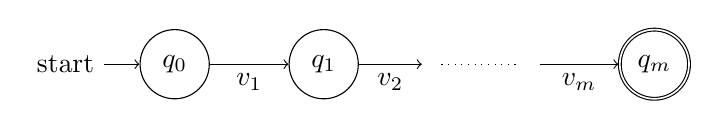
\begin{tikzpicture} 
		\node[state,initial] (q0)  {$q_0$};
		\node[state] (q1) [right = 1cm of q0] {$q_1$};
		\node (q2) [right = 0.8cm of q1]{};
		\node (q3) [right = 1cm of q2]{};
		\node[state,accepting] (qm) [right = 1cm of q3] {$q_m$};
		
		\draw[->] (q0) edge node [below]{$v_1$} (q1) ;
		\draw[->] (q1) edge node [below]{$v_2$} (q2) ;
		\draw[dotted] (q2) edge (q3) ;
		\draw[->] (q3) edge node [below]{$v_m$} (qm) ;
	\end{tikzpicture}}
. The corresponding integer constraint does not have exponential components. However, it does cover all numbers with at most $m$-digits. Consider the example $\sti{x}=10 \wedge |x|=5$. The number $10$ has only $2$-digits, at the first glance, a straight-line PFA with two transitions, i.e., the PFA
    \scalebox{0.5}{\tikzset{state/.style={circle,draw=blue!50,fill=blue!20,
			thick,inner sep=0pt,minimum size=6mm}, initial text=$ $}
	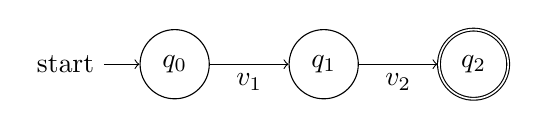
\begin{tikzpicture} 
	\node[state,initial] (q0)  {$q_0$};
	\node[state] (q1) [right = 1cm of q0] {$q_1$};
	\node[state,accepting] (q2) [right = 1cm of q1] {$q_2$};
	
	\draw[->] (q0) edge node [below]{$v_1$} (q1) ;
	\draw[->] (q1) edge node [below]{$v_2$} (q2) ;
	\end{tikzpicture}
	} should be sufficient for the domain restriction of $x$. If we do so, we will conclude that the formula is unsatisfiable, because the length of $x$ cannot be $5$  under this domain restriction.

However, the formula is satisfiable when $x=``00010"$. Observe that $\sti{``00010"}=10$. The key is that even for a bounded integer, the corresponding numeral can be of an unbounded length with arbitrarily many trailing `$0$'s at the front. All numbers with up to $m$-digits can be however still handled without having to solve exponential constraints. It is enough to equip the initial state of the PFA with a  $0$-self-loop.

Consequently, the automaton $A^m$ of our number PFA will have the following form illustrated in Figure~\ref{fig:sfa_its}. 
It has a self-loop on the initial state labeled by the character variable $v_0$, 
forced by the constraint 
$$
\Psi_{v_0}\defeq v_0=0
$$ 
to hold the value $0$. 
This transition ensures that the under-approximation handles numerals with arbitrary number of trailing zeros.  
The self-loop is followed by a chain of $m$ transitions $(q_{i-1},v_i,q_{i}),1\leq i \leq m$, leading towards the final state $q_m$. 
The chain encodes at most $m$ meaningful digits (only \emph{at most} because the first variables in the sequence can still be assigned zeros and some variables may be assigned $\epsilon$). Hence this PFA covers all numerals that encode numbers with at most $m$ digits.
Although it still has a loop, it will not create any exponential component defining the value of $n$ because the loop only represents a sequence of ``0'' at the front of $x$. It will not affect the integer value of $n=\sti{x}$.

\begin{figure}
	\scalebox{0.7}{
	\tikzset{state/.style={circle,draw=blue!50,fill=blue!20,
			thick,inner sep=0pt,minimum size=6mm}, initial text=$ $}
	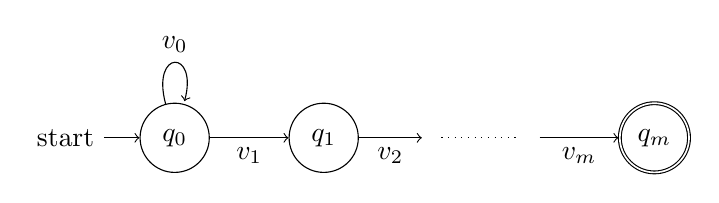
\begin{tikzpicture} 
	\node[state,initial] (q0)  {$q_0$};
	\node[state] (q1) [right = 1cm of q0] {$q_1$};
	\node (q2) [right = 0.8cm of q1]{};
	\node (q3) [right = 1cm of q2]{};
	\node[state,accepting] (qm) [right = 1cm of q3] {$q_m$};
	
	\draw[->] (q0) edge node [below]{$v_1$} (q1) ;
	\draw[->] (q1) edge node [below]{$v_2$} (q2) ;
	\draw[dotted] (q2) edge (q3) ;
	\draw[->] (q3) edge node [below]{$v_m$} (qm) ;
	\path (q0) edge [loop above] node {$v_0$} (q0);
	\end{tikzpicture} }
	
	\caption{PFA for string-number conversion constraints}
	\label{fig:sfa_its}
\end{figure}

%Such PFA handles bounded integers (e.g., 10-digits or 64-bits) precisely and under-approximate the possible values of unbounded integers. It works very efficiently because we just need to use linear constraints to characterize the relation between $x$ and $n$. 
Numeric PFA with these restrictions would satisfy our primary objective, that is, they would induce linear formulae and would ``easily'' and completely cover all numerals.
%
A last problem still needs to be solved beofe they can be efficient in practice. 
%
Recall that the character variables can be assigned $\epsilon$.  
%
Therefore, a single chain of $k$ interesting digits, $k\leq m$, can be by $A^m$ represented in $k\choose m$ ways, each corresponding to one possible interleaving of $k$ digits with $m-k$ epsilons. 
%
\lh{I am not sure whether it is really impossible to make a small formula}
%
This would lead to an exponential explosion of the size of the linear formula defining the value of $n$.
%
In order to eliminate this blow-up in the size of the formula, we add to $\paf^m$ an additional constraint that forces all epsilons to be \emph{shifted} behind the least significant digit, effectively prohibiting all interleavings but one. This is the formula
$$
\Psi_{\mathsf{shift}}^m \defeq \bigwedge_{1\leq i \leq m} v_i \neq \noepsilon \implies v_{i-1}\neq \noepsilon \ .
$$
Last, since this restriction is meaningful only when the string is indeed a numeral,  
we also define the constraint representing the strings which are not numerals, the formula
$$
\Psi_{\mathsf{NaN}}^m \defeq  \bigvee_{i\in [1,m]} v_i>9
$$ 
and define the final form of the interpretation restriction used by $A^m$ as 
$$
\paf^m \defeq  \Psi_{\mathsf{NaN}}^m \lor (\Psi_{v_0} \land \Psi_{\mathsf{shift}}^m)\ .
$$
Consequently, we design our domain restrictions $R$ so that for string variables $x$ that appear within string-integer constraints,  $R(x)$ is a number PFA $(A^m,\paf^m),m\in \nat$. 

Assuming that the domain restriction for $x$ is $(A^m,\paf^m)$, 
the value of the integer $n$ can be extracted from a numeral using the formula
$$
\Psi_{\mathsf{toInt}}^m\defeq \bigvee_{1\leq k \leq m} \Psi_{\mathsf{last(k)}}^m \land (n = v_1* 10^{k-1} + v_2* 10^{k-2} + \ldots + v_{k})
$$
where $\Psi_{\mathsf{last(k)}}^m$ says that the last variable of $A^m$ assigned a non-$\epsilon$ value is $v_{k}$, namely 
$$
\Psi_{\mathsf{last(k)}}^m \defeq (k = m \land v_k \geq 0) \lor (v_{k} \geq 0 \land v_{k+1} = -1)\ .
$$
Since we also need to distinguish the case when $x$ is not a number, in which case $n$ should equal $-1$, 
the formula underapproximating $\phi_s$ is finally constructed as  
\begin{multline*}
\underf R {\phi_s} 
\defeq 
\parikhfof{A^m} 
\land \\
\bigl((\Psi_{\mathsf{NaN}}^m \land n = -1) 
\lor 
(\neg\Psi_{\mathsf{NaN}}^m \land \Psi_{\mathsf{toInt}}^m)\bigr)
\end{multline*}
The following lemma states correctness of this construction:
\begin{lemma}
$
\semof {\underf R {\psi_s} }_{V_R \cup \#V_R \cup \{n\}} = \encode  R(\semof{\phi_s})
$
\end{lemma}



%
%
%$$
%\mathsf{toNumber(k)}\defeq (n = v_1\times 10^{k-1} + v_2\times 10^{k-2} + \ldots + v_{k})
%$$
%
%
%
%
%$$\Psi_{\mathsf{NaN}} \defeq  \bigvee_{i\in [1,m]} v_i>9$$
%where $ $
%To explain this encoding, we first define two macro function:
%
%$$\begin{array}{rl}
%\mathsf{epsilonAfter(k)}\defeq& (0\leq v_1,\ldots, v_k\leq 9) \wedge\\
%&v_{k+1}=\ldots =v_m = -1\\
%\mathsf{toNumber(k)}\defeq& (n = v_1\times 10^{k-1} + v_2\times 10^{k-2} + \ldots + v_{k})
%\end{array}
%$$

%The function $\mathsf{epsilonAfter(k)}$ forces the first $k$ variables to be assigned some number and those after $k$ be assigned $\epsilon$. Recall that we use $-1$ to represent $\epsilon$. The function $\mathsf{toNumber(k)}$ converts the first $k$ variables to the corresponding number in $n$. \yfc{say shifting $\epsilon$ to the right will not change the language}

%The condition that when $x$ is ``not a number'' is specified by the following formula.
%
%$$
%\Psi_{\mathit{NaN}} \defeq  \bigvee_{i\in [1,m]} v_i>9$$
%
%Then we can specify the relation between $n$ and the character variables as follows:
%$$\Psi_n\defeq  (n=-1 \wedge \Psi_{\mathit{NaN}})\vee \bigvee_{k\in [0,m]} (\mathsf{epsAfter(k)} \wedge \mathsf{toNumber(k)} )$$
%It says either $x$ is not a number and so $n=-1$ or the first $k$ variables represent the value of $n$, for some $k\in [0,m]$. 
%$$
%\underf R {\psi_s} \defeq \Psi_n \wedge \Psi_{v_0}\wedge \parikhfof {R(x)} 
%$$
%To formulate the correctness lemma similar to Lemmas~\ref{lemma:memcorrect} and \ref{lemma:eqcorrect}, we need to consider a modified semantics of $R(x)$.
%Namely, we assume that $\semof{R(x)}$ is returns $\decode A(\parikhof{R(x)} \land )$  



%We add $\Psi_n$ to $\Phi_O$.
%
%
%
%The correctness of this procedure is expressed in Lemma~\ref{lemma:sticorrect} below. We separate the lemmas to cases where $n\neq -1$ and $n=-1$. 
%
%
%\newcommand\restrict[1]{\raisebox{-.5ex}{$\big|$}_{#1}}


%\begin{lemma}\label{lemma:sticorrect}
%	
%	The interpretation $(I\cup\pim \cup I_n)  \in \semof {\Psi_n \wedge \Psi_{v_0}\wedge \parikhfof {A_x} }_{V_x \cup \#V_x \cup \{n\}} $ if and only if 
%	\begin{center}
%	 $\left(\begin{array}{c} 
%	 I_n(n)= \sti{\decode {A_x}(I\cup\pim)} \ \wedge \\
%	 I(v_i)=-1 \wedge i<j \Longrightarrow  I(v_j)=-1
%	 \end{array}\right)$\\ or\\
%	 $\left(\begin{array}{c} 
%	 I_n(n)= -1\ \wedge \decode {A_x}(I\cup\pim) \not\in [0,9]^+
%	 \end{array}\right)$
%	\end{center}
%
%\end{lemma}
%\yfc{sorry still ugly, the shifting of epsilon makes it a mess here}
%(An alternative description)
%\begin{lemma}\label{lemma:sticorrect}
%	For all $w \in \semof{A_{x}}$ and $c \in \mathbb{Z}$, we have 
%	\begin{center}
%		$\exists (I\cup\pim \cup I_n)  \in \semof {\Psi_n \wedge \Psi_{v_0}\wedge \parikhfof {A_x} }_{V_x \cup \#V_x \cup \{n\}}$ s.t. $w=\decode {A_x}(I\cup\pim)$ and $I_n(n)=c$\\
%		iff\\
%		$c= \sti{w}$.
%	\end{center}
%	
%\end{lemma}
%\hide{
%\begin{lemma}\label{lemma:sticorrect_pos}
%	$\semof {\Psi_n \wedge \Psi_{v_0}\wedge \parikhfof {A_x} }_{V_x \cup \#V_x \cup \{n\}} = \{(I\cup\pim \cup I_n) \mid  I_n(n)= \sti{\decode {A_x}(I\cup\pim)}\} $. 
%\end{lemma}
%In this case, $x$ encodes a number. The lemma says when the models we add to $\Phi_O$ represents a word in $\semof{A_x}$ whose integer value is exactly the model for $n$.
%
%\begin{lemma}\label{lemma:sticorrect_neg}
%	$\semof {\Psi_n \wedge \parikhfof {A_x} \wedge (v_0 = 0)\wedge (n = -1) }_{V_x \cup \#V_x \cup \{n\}} = 
%	\{(I\cup\pim \cup I_n) \mid  I_n(n)= -1 \wedge \decode {A_x}(I\cup\pim) \not\in [0,9]^+  \}$
%\end{lemma}
%
%In this case, $x$ does not encode a number. The lemma says  the models we add to $\Phi_O$ represents words in both $\semof{A_x}$ and $[0,9]^+$, which means not a number, and $n$ is $-1$.}
%
%\lh{
%\begin{lemma}
%$
%\semof {\Psi_n \wedge \Psi_{v_0}\wedge \parikhfof {A_x} }_{V_x \cup \#V_x \cup \{n\}} = \encode  R(\semof{\phi_s})
%$
%\end{lemma}
%The $n$ must somehow be handled properly by $\encode  R(\phi_s)$, I did not have time to think about it yet.
%}



% \section{Evaluation}
% \label{section:evaluation}
% \todo{copy a few tables from our test site to here}




\section{Implementation and Evaluation}
\label{section:evaluation}

We have implemented our string constraint solving procedure in a tool called {\tool}. {\tool} is implemented as a theory solver of the SMT solver Z3~\cite{z3}. In this way, we can concentrate on solving conjunctive constraints and let Z3 handle the other boolean connectives. Secondly, it makes it possible to solve not only formulae over string constraints but also combinations of string constraints with other theories that Z3 supports. Furthermore, this approach allows us to more effectively handle the arithmetic constraints that are generated by the under-approximation module and, lastly, it eliminates the need to have our own parser. 

In {\tool}, we use the following PFA selection strategy. We use \emph{numeric PFAs} for string variables appearing in string-number conversion and \emph{standard PFAs} for others. We select a size $m$ for numeric PFAs, a number $p$ of their loops, and the length $q$ of the loops. Initially, we set $(m,p,q)=(5,2,q)$ where $q$ is dynamic and obtained from our internal static analysis. We double $m$ and increase $p$ and $q$ by one if refinement is required. We set an upper bound for each parameter and report UNKNOWN if a solution cannot be found within the bound.

Our over-approximation module also uses heuristics to derive the constant value of any side of the constraint $n=\sti{x}$ to refine the over-approximation. For instance, assume we can derive that $n=12$ from some integer constraints. Then we can derive the value of $x$ belongs to the regular language $(0^*12)$. 
%HERE

%more or less standard
The way our theory solver and Z3 interact is almost standard. When Z3 asks our theory solver a string constraint satisfiability problem, our solver tries to prove it is SAT or UNSAT using the procedure discussed in this paper. For under-approximation, whenever a corresponding linear formula is created, we attach the current value of $m$, $p$, $q$ to the formula, and then push it to Z3 core. If our theory solver reports UNKNOWN, Z3 remembers it in a global flag \textsf{incomplete} and either tries another solution branch, or the same solution branch with different value of $m$, $p$, $q$. If Z3 completes the search of all solution branches, it reports UNSAT if the flag \textsf{incomplete} is down, and UNKNOWN otherwise.


We compare {\tool} \changed{(\texttt{1e715b7dab})} with other state-of-the-art string solvers, namely, CVC4~(45bcf28ab)~\cite{cvc4Tool}, and Z3~(\texttt{d95b549ff})~\cite{z3}, \textsf{Z3Str3}~(\texttt{d95b549ff})~\cite{zheng2013z3}. For these tools, we use the GitHub version stated in the parenthesis because their performance are in general better than the corresponding release version. \changed{Observe that CVC4 and Z3 are  DPLL(T)-based string solvers.}
We do not compare with Sloth \cite{sloth} since it does not support length constraints, which occur in most of our benchmarks. We also do not compare with ABC~\cite{aydin2018parameterized} (a model counter for string constraints), Ostrich~\cite{chen2019decision} and \textsf{Trau+}~\cite{abdulla2019chain}, because they do not support many of the string functions in our benchmarks, especially string-number conversion.

We perform two sets of experiments. In the first set of experiments, we compare {\tool} with other tools on existing benchmarks over basic string constraints. Those benchmarks do not involve string-number conversion functions. In the second set of experiments, we compare {\tool} with the other tools on new suites focusing on string-number conversion. Our goals of experiments are the following:
\smallskip


\begin{itemize}
	\item {\tool} performs as good as or better than the other tools in solving the  satisfiability problems of basic string constraints.
	
		\smallskip

	\item {\tool} performs significantly better than the other tools in solving the satisfiability problems on string-number conversion benchmark, and this shows  the efficiency of PFA in general and \emph{numeric} PFA in particular.
\end{itemize}
		\smallskip

In the first set of experiments, we use the following benchmark examples:

		\smallskip


\begin{itemize}
	\item PyEx~\cite{pyex} comes from running the symbolic executor PyEx over some Python packages.
	
	\smallskip
	
	
%	\item APLAS~\cite{aplas} includes 600 hand-drafted tests consisting of only equality and integer length constraints.
	
	
	%	\smallskip


	\item \changed{ LeetCode comes from running PyEx over a sample code collected from the LeetCode~\cite{LeetCode} website, including functions that check whether a string is a valid IPv4 or IPv6 address, sum up two binary numbers, check whether an input string is an abbreviation of another input string, and convert a sequence of digits to a string according to a given mapping.}
	
		\smallskip

	\item StringFuzz~\cite{blotsky2018stringfuzz}  is generated by the fuzz testing tool of the same name.
	
		\smallskip

	\item $\text{cvc4}_{\text{pred}}$ and $\text{cvc4}_{\text{term}}$ are obtained from the CVC4 group~\cite{termEQ}. These benchmarks contain a small amount of string-number conversion constraints (< $5\%$).
\end{itemize}

In the second experiment, we compare with tools supporting string-number conversion on the benchmarks collected from the symbolic executor \texttt{Py-Conbyte}\footnote{\url{https://github.com/spencerwuwu/py-conbyte}}, which has the supports of string-number conversion. We ran it on several examples collected from the LeetCode platform and from Python core libraries, which involve diverse usages of string-number conversion in Python such as parsing date-time, verifying and restoring IP addresses from strings, etc. We also have examples that encode execution paths of some JavaScript programs (the Luhn algorithm and some array manipulations).

	\changed{All experiments were executed on a machine with 4-core CPU, 16 GiB RAM, and MacOS 10.15.4.} The timeout was set to 10s for each test.
We use the results from {\tool}, CVC4, and Z3 as the reference answer for the validation of the correctness of the results. Occasionally, two of them report inconsistent  answers (one SAT and one UNSAT). To decide which solver is right, we developed a validator. It takes the model $I$ returned from the solver who reported SAT, assigns $I(x)$ to all variables $x$ in the test to obtain a modified test, and re-evaluates the modified test by multiple solvers. If the results from all solvers are consistent, we mark the test SAT or UNSAT according to the results. Otherwise, we manually simplify and inspect the test until we get a conclusive result. 

\changed{The results of the experiments are summarized in Table~\ref{table:base_benchmark}, Table~\ref{table:str_int_benchmark}, and Table~\ref{table:checkLuhn}. Rows with heading \texttt{SAT}/\texttt{UNSAT} show numbers of solved formulae. Rows with heading \texttt{UNKNOWN} or \texttt{TIMEOUT} indicate the number of instances for which the solver fails to return an answer. \texttt{ERROR} means system crashes due to various reasons (usually out of memory). \texttt{INCORRECT} shows the number of cases where the tool gives a wrong answer.}


\begin{table}[h]
\changed{
\centering
\caption{Results of {\tool}, CVC4, Z3, and Z3Str3 on Basic String Constraint benchmarks.}
\scalebox{0.85}{
\begin{tabular}{|l r | r r r r |}
\hline
\multicolumn{2}{|c}{}                  & {\tool} & CVC4  &Z3 & Z3Str3 \\ \hline
\multirow{6}{*}{PyEx}		& SAT      & 21377& 19899& 16331&  3037 \\
							& UNSAT    &  3860&  3848&  3831&  3816 \\
							& UNKNOWN  &     0&     0&     0&     7 \\
							& TIMEOUT  &   184&  1674&  5259& 16872 \\
							& ERROR    &     0&     0&     0&  1675 \\
							& INCORRECT&     0&     0&     0&    14 \\ \hline
%\multirow{6}{*}{APLAS}		& SAT      &   126&    51&    13&    35 \\
%							& UNSAT    &   286&   214&   100&   111 \\
%							& UNKNOWN  &     0&     0&     0&   345 \\
%							& TIMEOUT  &   188&   335&   487&    89 \\
%							& ERROR    &     0&     0&     0&    20 \\
%							& INCORRECT&     0&     0&     0&     0 \\ \hline
\multirow{6}{*}{LeetCode}	& SAT      &   877&   865&   881&   661 \\
							& UNSAT    &  1785&  1785&  1785&  1780 \\
							& UNKNOWN  &     0&     0&     0&   122 \\
							& TIMEOUT  &    0&    16&     0&    90 \\
							& ERROR    &     4&     0&     0&    13 \\
							& INCORRECT&     0&     0&     0&     0 \\ \hline
\multirow{6}{*}{StringFuzz}	& SAT      &   515&   704&   267&   505 \\
							& UNSAT    &   301&   245&   188&   192 \\
							& UNKNOWN  &     0&     0&     0&     4 \\
							& TIMEOUT  &   249&   116&   610&   364 \\
							& ERROR    &     0&     0&     0&     0 \\
							& INCORRECT&     0&     0&     0&     0 \\\hline
\multirow{6}{*}{cvc4\textsubscript{pred}} & SAT &    13&    11&    12&     8 \\
							& UNSAT    &   822&   818&   808&   774 \\
							& UNKNOWN  &     0&     0&     0&     4 \\
							& TIMEOUT  &     0&     6&    15&    38 \\
							& ERROR    &     0&     0&     0&     11 \\
							& INCORRECT&     0&     0&     0&     0 \\ \hline
\multirow{6}{*}{cvc4\textsubscript{term}} & SAT &    10&     8&     5&    2 \\
							& UNSAT    &  1032&  1025&  1022&   957 \\
							& UNKNOWN  &     0&     0&     0&     3 \\
							& TIMEOUT  &     3&    12&    18&    58 \\
							& ERROR    &     0&     0&     0&     11 \\
							& INCORRECT&     0&     0&     0&    14 \\ \hline \hline
\multirow{6}{*}{Total} 		& SAT      & 22792& 21487& 17496&  4213\\
							& UNSAT    &  7800&  7721&  7634&  7519\\
							& UNKNOWN  &     0&     0&     0&   140\\
							& TIMEOUT  &  436&  1824&  5902& 17422 \\
							& ERROR    &     4&     0&     0&  1710\\
							& INCORRECT&     0&     0&     0&    28 \\\hline
\end{tabular}}
\label{table:base_benchmark}}
\end{table}

\begin{table}[h]
\changed{
\centering
\caption{Results of {\tool}, CVC4, Z3, and Z3Str3 on String-Number Conversion benchmark.}
\scalebox{0.8}{
\begin{tabular}{|l r | r r r r|}
\hline
\multicolumn{2}{|c}{}          			   & {\tool} &  CVC4 &    Z3 & Z3Str3 \\ \hline
\multirow{6}{*}{Leetcode}		& SAT      &  2501&  1721&  1898&   239 \\ 
								& UNSAT    & 16394& 15726& 16115& 15288 \\
								& UNKNOWN  &     0&     0&     0&   623 \\
								& TIMEOUT  &    32&  1480&   914&  2337 \\
								& ERROR    &     0&     0&     0&   332 \\
								& INCORRECT&     0&     0&     0&   108 \\ \hline 
\multirow{6}{*}{PythonLib}		& SAT      &  1922&   579&   914&   206 \\ 
								& UNSAT    &   724&   667&   724&   642 \\
								& UNKNOWN  &     0&     0&     0&    45 \\
								& TIMEOUT  &     0&  1400&  1008&  1710 \\
								& ERROR    &     0&     0&     0&    41 \\
								& INCORRECT&     0&     0&     0&     2 \\ \hline
\multirow{6}{*}{JavaScript}		& SAT      &    20&     3&    16&     4 \\ 
								& UNSAT    &     0&     0&     0&     0 \\
								& UNKNOWN  &     0&     9&     0&     0 \\
								& TIMEOUT  &     0&     8&     4&    10 \\
								& ERROR    &     0&     0&     0&     6 \\
								& INCORRECT&     0&     0&     0&     0 \\ \hline \hline
\multirow{6}{*}{Total}			& SAT      &  4443&  2303&  2828&   449 \\ 
								& UNSAT    & 17118& 16393& 16839& 15930 \\
								& UNKNOWN  &     0&     9&     0&   668 \\
								& TIMEOUT  &    32&  2888&  1926&  4057 \\
								& ERROR    &     0&     0&     0&   379 \\
								& INCORRECT&     0&     0&     0&   110 \\ \hline
\end{tabular}}
\label{table:str_int_benchmark}
}
\end{table}


% \begin{table}[h]
% \centering
% \caption{Results of {\tool}, CVC4, Z3, and Z3Str3 on Basic String Constraint benchmarks.}
% \scalebox{0.85}{
% \begin{tabular}{|l r | r r r r |}
% \hline
% \multicolumn{2}{|c}{}                  & {\tool} & CVC4  &Z3 & Z3Str3 \\ \hline
% \multirow{3}{*}{PyEx}		& SAT      &  19468  & 19763 & 16528 &  3030 \\ 
% 							& UNSAT    &   3854  &  3834 &  3831 &  3836 \\
% 							& $\times$ &   2099  &  1824 &  5062 & 18555 \\ \hline
% \multirow{3}{*}{APLAS}		& SAT      &    131  &   205 &    12 &    37 \\
% 							& UNSAT    &    288  &   221 &   100 &   111 \\
% 							& $\times$ &    181  &   174 &   488 &   452 \\ \hline
% \multirow{3}{*}{LeetCode}	& SAT      &    881  &   859 &   881 &   670 \\
% 							& UNSAT    &   1785  &  1785 &  1785 &  1780 \\
% 							& $\times$ &      0  &    22 &     0 &   216 \\ \hline
% \multirow{3}{*}{StringFuzz}	& SAT      &    498  &   671 &   264 &   491 \\
% 							& UNSAT    &    319  &   240 &   186 &   192 \\
% 							& $\times$ &    248  &   154 &   615 &   382 \\\hline
% \multirow{3}{*}{cvc4\textsubscript{pred}} & SAT & 11 & 11 &   12 &     8 \\
% 							& UNSAT    &    820  &   818 &   808 &   772 \\
% 							& $\times$ &      4  &     6 &    15 &    55 \\ \hline
% \multirow{3}{*}{cvc4\textsubscript{term}} & SAT & 13 & 8 &     5 &    17 \\
% 							& UNSAT    &   1031  &   936 &  1021 &   958 \\
% 							& $\times$ &      1  &   101 &    19 &    70 \\ \hline \hline
% \multirow{3}{*}{Total} 		& SAT      &  21002  & 21517 & 17702 &  4253 \\
% 							& UNSAT    &   8097  &  7834 &  7731 &  7649 \\
% 							& $\times$ &   2533  &  2281 &  6199 & 19730 \\\hline	
% \end{tabular}}
% \label{table:base_benchmark}
% \end{table}

% \begin{table}[h]
% \centering
% \caption{Results of {\tool}, CVC4, Z3, and Z3Str3 on String-Number Conversion benchmark.}
% \scalebox{0.8}{
% \begin{tabular}{|l r | r r r r|}
% \hline
% \multicolumn{2}{|c}{}          			   & {\tool} & CVC4  &    Z3  & Z3Str3 \\ \hline
% \multirow{3}{*}{Leetcode}		& SAT      &   2349  &  1543 &  1892  &   217 \\ 
% 								& UNSAT    &  16368  & 15676 & 16105  & 15374 \\
% 								& $\times$ &    210  &  1708 &   930  &  3336 \\ \hline 
% \multirow{3}{*}{PythonLib}		& SAT      &    886  &   408 &   797  &   201 \\ 
% 								& UNSAT    &    720  &   660 &   724  &   644 \\
% 								& $\times$ &   1040  &  1578 &  1125  &  1801 \\ \hline
% \multirow{3}{*}{JavaScript}		& SAT      &     20  &     6 &    16  &     4 \\ 
% 								& UNSAT    &      0  &     0 &     0  &     0 \\
% 								& $\times$ &      0  &    14 &     4  &    16 \\ \hline \hline
% \multirow{3}{*}{Total}			& SAT      &   3255  &  1957 &  2705  &   422 \\ 
% 								& UNSAT    &  17088  & 16336 & 16829  & 16018 \\
% 								& $\times$ &   1250  &  3300 &  2059  &  5153 \\ \hline
% \end{tabular}}
% \label{table:str_int_benchmark}
% \end{table}


From Table~\ref{table:base_benchmark}, we can see that the performance of {\tool} is as good as that of the most competitive tools such as CVC4 and Z3 on basic string constraints. In all of the benchmarks, {\tool} ranked either the 1st or the 2nd on the number of solved (SAT+UNSAT) cases. On the StringFuzz benchmarks that are SAT, {\tool} does not perform as well as the best performing tool. We however do not consider this crucial because these benchmarks are just randomly generated for debugging. On the most important benchmarks, those that come from program analysis, {\tool} is comparable to the best performing tool.

%\changed{
%From Table~\ref{table:str_int_benchmark}, we can see that {\tool} significantly outperforms all the other tools. 
%The second best tool, Z3, fails on 38\% more examples. 
%}
\changed{
From Table~\ref{table:str_int_benchmark}, we can see that {\tool} significantly outperforms all the other tools. 
The second best tool, Z3, fails on 50 times more examples. 
}
%It fails on twice less cases then Z3, which is ranked the 2nd. In fact, most of the failed tests come from the analysis of one Python core library function that converts an IPv6 address to a number. From around 2028 tests generated from this function, around 1000 tests are too difficult for all solvers.  If we exclude the 2028 tests generated from this function, then {\tool} has only $218$ failed cases in total. This is significantly better than the 2nd place tool Z3, which fails on $942$ cases in total.

%We also ran experiments on the String-Number Conversion benchmark with the timeout set to 30s. Provided more time for solving, {\tool} managed to obtain more results and the number of failed cases is reduced to 539, while CVC4 and Z3Str3 got almost the same number of failed cases. Z3 also managed to reduce the number of failed cases to 821. %If we exclude results on the Python core function that converts an IPv6 address to a number mentioned above, {\tool} has only $53$ timeouts in total while z3 has $809$ in total.

As an addition experiment, we have encoded the checkLuhn algorithm introduced in Section~\ref{section:introduction} for the cases with 2 to 12 loops (digits). We ran these tests 
%additionally to the experiments above 
with the timeout set to 120s. The result is summarized in Table~\ref{table:checkLuhn}.
In these tests, {\tool} can solve all problems within 1s while CVC4 only returns a model for cases of 2 to 5 loops and Z3Str3 could not solve any of these problems (either timeout or UNKNOWN). However, Z3 can still solve 7 out of the 11 problems, while timeouting in the cases with 4, 5, 7, and 9 loops. The behavior of Z3 is not entirely unexpected. All the problems are satisfiable and the solver may be lucky to guess the solution quickly. % branch with a correct model quickly.

\begin{table}[h]
\changed{

\centering
\caption{Comparison of {\tool}, CVC4, Z3, and Z3Str3 with checkLuhn problems of 2 to 12 loops.}
\scalebox{0.8}{
\begin{tabular}{| c | c c c c|}
\hline
\# of Loops & {\tool} 			   &  CVC4    	 		  &       Z3   			& Z3Str3 \\ \hline
2 			& \textbf{SAT}(0.27s)  &  \textbf{SAT}(0.89s) & \textbf{SAT}(0.45s) & \textbf{ERROR} \\
3  			& \textbf{SAT}(0.29s)  &  \textbf{SAT}(1.17s) & \textbf{SAT}(0.10s) & \textbf{ERROR} \\
4 			& \textbf{SAT}(0.37s)  &  \textbf{SAT}(4.92s) & \textbf{TIMEOUT}    & \textbf{ERROR} \\
5 			& \textbf{SAT}(0.39s)  &  \textbf{SAT}(11.27s)& \textbf{TIMEOUT}    & \textbf{ERROR} \\
6 			& \textbf{SAT}(0.41s)  &  \textbf{TIMEOUT}    & \textbf{SAT}(0.13s) & \textbf{UNKNOWN} \\
7 			& \textbf{SAT}(0.51s)  &  \textbf{TIMEOUT}    & \textbf{TIMEOUT}    & \textbf{ERROR} \\
8 			& \textbf{SAT}(0.53s)  &  \textbf{TIMEOUT}    & \textbf{SAT}(0.29s) & \textbf{ERROR} \\
9 			& \textbf{SAT}(0.63s)  &  \textbf{TIMEOUT}    & \textbf{TIMEOUT}    & \textbf{ERROR} \\
10 			& \textbf{SAT}(0.69s)  &  \textbf{TIMEOUT}    & \textbf{SAT}(0.48s) & \textbf{TIMEOUT} \\
11 			& \textbf{SAT}(0.71s)  &  \textbf{TIMEOUT}    & \textbf{SAT}(0.36s) & \textbf{ERROR} \\
12 			& \textbf{SAT}(0.74s)  &  \textbf{TIMEOUT}    & \textbf{SAT}(0.38s) & \textbf{TIMEOUT} \\ \hline
\end{tabular}}
\label{table:checkLuhn}}
\end{table}


% \todo{Update table with data of timeout=30s}

% \begin{table}[h]
% \centering
% \caption{Comparison of {\tool}, CVC4, Z3, and Z3Str3 with checkLuhn problems of 2 to 12 loops.}
% \scalebox{0.9}{
% \begin{tabular}{| c | c c c c|}
% \hline
% \# of Loops & {\tool} 			   &  CVC4    	 		  &       Z3   			& Z3Str3 \\ \hline
% 2 			& \textbf{SAT}(<0.1s)  &  \textbf{SAT}(0.66s) & \textbf{SAT}(0.23s) & $\times$ \\
% 3  			& \textbf{SAT}(<0.1s)  &  \textbf{SAT}(1.78s) & \textbf{SAT}(0.13s) & $\times$ \\
% 4 			& \textbf{SAT}(<0.1s)  &  \textbf{SAT}(6.96s) &   $\times$  		& $\times$ \\
% 5 			& \textbf{SAT}(<0.1s)  &  \textbf{SAT}(17.2s) &   $\times$  		& $\times$ \\
% 6 			& \textbf{SAT}(0.16s)  &  $\times$  		  & \textbf{SAT}(0.14s) & $\times$ \\
% 7 			& \textbf{SAT}(0.24s)  &  $\times$    		  &   $\times$  		& $\times$ \\
% 8 			& \textbf{SAT}(0.31s)  &  $\times$   		  & \textbf{SAT}(0.37s) & $\times$ \\
% 9 			& \textbf{SAT}(0.26s)  &  $\times$    		  &   $\times$  		& $\times$ \\
% 10 			& \textbf{SAT}(0.21s)  &  $\times$    		  & \textbf{SAT}(0.62s) & $\times$ \\
% 11 			& \textbf{SAT}(0.23s)  &  $\times$    		  & \textbf{SAT}(0.47s) & $\times$ \\
% 12 			& \textbf{SAT}(0.33s)  &  $\times$     		  & \textbf{SAT}(0.47s) & $\times$ \\ \hline
% \end{tabular}}
% \label{table:checkLuhn}
% \end{table}


\hide{
\paragraph{Basic constraint benchmarks.}
This group of benchmarks consists of PyEx, APLAS, LeetCode, StringFuzz, cvc4\textsubscript{pred} and cvc4\textsubscript{term}, which are benchmarks that were obtained by using an existing tool or generated by other groups. In this group of benchmarks, we would like to show that the performance of our tools is not only comparable to the performance of other tools, but in some cases even better.

The first benchmark is called PyEx~\cite{pyex} according to the same-named tool, which is a symbolic executor designed for Python developers to achieve high-coverage testing. This benchmark was obtained from the CVC4 group who ran PyEx on a test suite from 4 popular Python packages: httplib2, pip, pymongo, and requests. PyEx benchmark consists of 25421 tests which contain formulae with diverse string constraints.

The second benchmark is called APLAS that was created by authors of \textsf{$Kepler_{22}$}~\cite{aplas}. The benchmark includes a total of 600 hand-crafted tests (298 satisfiable and 302 unsatisfiable) involving looping word equations (Both sides of the string equality have a common variable) and length constraints over strings. 

The next benchmark is called LeetCode~\cite{LeetCode} that was obtained by extracting constraints from Python's testing solutions provided by LeetCode platform. They provide many programming examples and their solutions gathered from technical interviews for companies. Leetcode consists of 881 satisfiable and 1785 unsatisfiable tests that, like PyEx, contain diverse string constraints.

StringFuzz is our next benchmark that is named after a fuzzer~\cite{StringFuzz} for automatically generating SMT-LIB string constraints. We used StringFuzz to generate 1065 tests including word (dis)equalities, regular membership and arithmetic constraints. 

The last two benchmarks, called $\text{cvc4}_{\text{pred}}$ and $\text{cvc4}_{\text{term}}$, are obtained from cvc4 group~\cite{termEQ}. This set of benchmarks consists of the verification of term equivalences over strings and includes various string constraints including string-number and number-string conversion constraints.


\paragraph{String-number conversion constraint benchmarks.}
Our second group of benchmarks was created in order that we could compare our proposed approach for solving string-number and number-string conversions with existing approaches. This group contains a total of 3 benchmarks: full\_str\_int, filtered\_str\_int and rec\_fun. None of these benchmarks were artificially generated but were created from real Python's and javascript's codes.

The first benchmark in the group is full\_str\_int, which is a collection of SMT queries. This collection was generated by applying a tool for concolic testing to Python codes selected from the previously mentioned LeetCode platform and from Python core libraries. All selected Python codes use the \texttt{int()} function, which converts a string into a number system based on the specified base. The Benchmark consists of 21573 tests in total.

The second benchmark, called filtered\_str\_int, is a subset of the previous full\_str\_int benchmark. The filtered\_str\_int benchmark was created by removing tests where cvc4 reported UNSAT and where cvc4's returned unsat core contained no conversion constraint. This benchmark was created in order that we better compare individual conversion approaches. A total of 7396 tests were left.

The last benchmark in the group is rec\_fun, which is a collection of javascript functions that were handcrafted encoded into smt2 format using recursive functions. Besides running examples from the introduction, the benchmark also includes \texttt{split} and \texttt{replaceAll} functions. In total, we managed to create 43 tests that combine several SMT theory and contain conversion constrains.
}

\hide{
In this section, we compare our implementation z3-Trau with other SMT tools cvc4, z3, and Z3Str3 as evauation. To show the general performance of z3-Trau, we compare z3-Trau with other string solvers on selected string benchmarks: PyEx is a benchmark obtained from symbolic execution of Python code[]; APLAS is a benchmark involving looping word equations[]; 
LeetCode is obtiained from concolic testing LeetCode solutions written in Python code; StringFuzz is a benchmark of instance SMT-lib string problems generated by StringFuzz generator tool[]; cvc4\textsubscript{pred} and cvc4\textsubscript{term} are benchmarks provided by the cvc4 development team[]. Table~\ref{table:base_benchmark} shows the result of the comparison. \changed{The experiments are conducted with a machine of the following specifications: 4-core CPU, 16GB RAM, MacOS 10.15.4.} We set the timeout is to 10 seconds. Because the amount of problems is very large, we ran these experiments separately on several machines with the same specification on a computer cluster. The results are either sat, unsat, timeout, or $\times$. In case $\times$, the result may be unknown, error, or exception.


\textbf{Comparison according to Table 1......}

To evaluate our strategy for string-number/number-string conversion, we also prepared a benchmark \texttt{str\_int}\footnote{\url{https://github.com/plfm-iis/str_int_benchmarks}}. It is collected from two sources of Python programs that use ttexttt{int()} function: Leetcode solutions written in Python and Python core libraries. We concolic tested these Python programs by \texttt{Py-Conbyte}\footnote{\url{https://github.com/spencerwuwu/py-conbyte}}, our concolic tester for Python programs. The SMT queries during the concolic testing are collected as our benchmark. To be more precise in evalutation, we have two versions of \texttt{str\_int} benchmark: \texttt{full\_str\_int} and \texttt{filtered\_str\_int}. \texttt{full\_str\_int} is the original benchmark we collected (i.e. from Python programs using \texttt{int()}); \texttt{filtered\_str\_int} is a subset of \texttt{fill\_str\_int}. We filtered out problems that cvc4 says unsat while the unsat cores do not contain \texttt{str.to.int} or \texttt{int.to.str}. The results of experiment on \texttt{str\_int} benchmark is listed in Table~\ref{table:str_int_benchmark}. The experiments are conducted under the same condition as the experiments on other benchmarks.

\textbf{Comparison according to Table 2.....}
}



\hide{
\begin{table}[]
\caption{Results of z3-Trau, cvc4, and z3 on full\_str\_int benchmark}
\begin{tabular}{|r|r|r|r|r|r|r|}
\hline
Tool		& sat & unsat & u.k. & t.o. & err. & misc \\ \hline\hline
z3-Trau		& 3289 & 17089 & 0 & 1195 & 0 & 0 \\ 
cvc4		& 2185 & 16377 & 0 & 3011 & 0 & 0 \\ 
z3seq		& 2716 & 16831 & 0 & 2026 & 0 & 0 \\ 
Z3Str3		& 422 & 16034 & 634 & 4131 & 347 & 5 \\ \hline
\end{tabular}
\label{table:full_str_int}
\end{table}

Table~\ref{table:filtered_str_int} shows the comparison on filtered\_str\_int.  The total amount of cases in filtered\_str\_int is 7396.

\begin{table}[]
\caption{Results of z3-Trau, cvc4, and z3 on filtered\_str\_int benchmark}
\begin{tabular}{|r|r|r|r|r|r|r|}
\hline
Tool		& sat & unsat & u.k. & t.o. & err. & misc \\ \hline\hline
z3-Trau		& 3281 & 2912 & 0 & 1203 & 0 & 0 \\ 
cvc4		& 2210 & 2211 & 0 & 2975 & 0 & 0 \\ 
z3seq		& 2729 & 2655 & 0 & 2012 & 0 & 0 \\ 
Z3Str3		& 424 & 1944 & 587 & 4106 & 330 & 5 \\ \hline
\end{tabular}
\label{table:filtered_str_int}
\end{table}
}





\hide{ % keep data of abc and ostrich
\begin{table}[h]
\centering
\caption{Results of Z3-Trau, CVC4, and Z3 on Basic String Constraint benchmarks (numbers with * will be updated later)}
\scalebox{0.7}{
\begin{tabular}{|l r | r r r r r r r|}
\hline
\multicolumn{2}{|c}{}                   & {\tool} & CVC4  &Z3 & Z3Str3 & Trau+ & ABC & Ostrich \\ \hline
\multirow{3}{*}{PyEx}		& sat      & 19586*   & 19763* & 18490 &   3024*  & 19149 & 0 & 111 \\ 
							& unsat    &  3858*   &  3834* &  3855 &   3839*  & 3828 & 0 & 871 \\
							& $\times$ &  1977*   &  1824* &  3076 &  18558*  & 2444 & 25421 & 24439 \\ \hline
\multirow{3}{*}{APLAS}		& sat      &   128*   &   205* &    19 &     38*  & 132 & 289 & 0 \\
							& unsat    &   287*   &   211* &   100 &    111*  & 82 & 2 & 1 \\
							& $\times$ &   185*   &   174* &   481 &    451*  & 386 & 309 & 599 \\ \hline
\multirow{3}{*}{LeetCode}	& sat      &   856*   &   860* &   881 &    670*  & 778 & 0 & 158 \\
							& unsat    &  1784*   &  1785* &  1785 &   1780*  & 1827 & 0 & 1618 \\
							& $\times$ &    26*   &    21* &     0 &    216*  & 61 & 2666 & 890 \\ \hline
\multirow{3}{*}{StringFuzz}	& sat      &   502*   &   677* &   316 &    493*  & 688 & 439 & 0 \\
							& unsat    &   294*   &   240* &   206 &    190*  & 339 & 158 & 0 \\
							& $\times$ &   269*   &   148* &   543 &    382*  & 38 & 468 & 1065 \\\hline
\multirow{3}{*}{cvc4\textsubscript{pred}} & sat & 16* & 11* &   12 &      8*  & 247 & 316 & 21 \\
							& unsat    &   814*   &   818* &   807 &    772*  & 500 & 443 & 17 \\
							& $\times$ &     5*   &     6* &    16 &     55*  & 88 & 76 & 797 \\ \hline
\multirow{3}{*}{cvc4\textsubscript{term}} & sat & 13* & 8* &     6 &     16*  & 311 & 576 & 45 \\
							& unsat    &  1030*   &   936* &  1020 &    958*  & 596 & 349 & 22 \\
							& $\times$ &     2*   &   101* &    19 &     71*  & 137 & 120 & 978 \\ \hline
\multirow{3}{*}{SLOG}  		& sat      & 0* & 1309* & 0 & 0* & 1228 & 1036 & 1299 \\
							& unsat    & 3391* & 2082* & 2824 & 2205* & 2079 & 1972 & 2079 \\
							& $\times$ & 0* & 0* & 567 & 1186* & 84 & 383 & 13 \\ \hline \hline
\multirow{3}{*}{Total} 		& sat      & * & * & 19724 & * &  &  &  \\
							& unsat    & * & * & 10597 & * &  &  &  \\
							& $\times$ & * & * &  4702 & * &  &  &  \\\hline
\end{tabular}}
\label{table:base_benchmark}
\end{table}
}


\hide{ %3rd version of tables
\begin{table}[t]
	\centering
	\caption{Results of {\tool}, cvc4, and z3 on str\_int benchmark (numbers with * will be updated later)}
	\scalebox{0.7}{
		\begin{tabular}{l r | r r r r}
			\hline
			\multicolumn{2}{c}{}                   & {\tool} & CVC4   &    Z3  & Z3Str3 \\ \hline
			\multirow{3}{*}{String-Number}		& sat      &   3294*  &  2185* &  2731* &    422* \\ 
			& unsat    &  17088*  & 16377* & 16832* &  16034* \\
			& $\times$ &   1191*  &  3011* &  2010* &   5117* \\ \hline \hline 
				
				\multirow{3}{*}{leetcode-addStrings}	& sat & 622*  &  330* &  100* &  85* \\ 
				& unsat    &  1054*  & 780* & 1043* &  634* \\
				& $\times$ &  2*  &  568* &  535* & 959* \\ \hline
				\multirow{3}{*}{leetcode-add\_Binary}	& sat & 520*  &  530* &  531* &  11* \\ 
				& unsat    &  1351*  & 1091* & 1091* &  1094* \\
				& $\times$ &  11*  &  261* &  260* & 777* \\ \hline
				\multirow{3}{*}{leetcode-numDecodings}	& sat & 166*  &  107* &  151* &  50* \\ 
				& unsat    &  273*  & 269* & 283* &  269* \\
				& $\times$ &  92*  &  155* &  97* & 212* \\ \hline
				\multirow{3}{*}{leetcode-restoreIpAddresses}	& sat & 811*  &  462* &  864* &  55* \\ 
				& unsat    &  13648*  & 13540* & 13648* &  13342* \\
				& $\times$ &  54*  &  511* &  1* & 1116* \\ \hline
				\multirow{3}{*}{leetcode-validIPAddress}	& sat & 54*  &  57* &  58* &  8* \\ 
				& unsat    &  19*  & 19* & 19* &  19* \\
				& $\times$ &  4*  &  1* &  0* & 50* \\ \hline
				\multirow{3}{*}{leetcode-validWordAbbreviation}	& sat & 183*  &  193* &  188* &  8* \\ 
				& unsat    &  24*  & 11* & 21* &  16* \\
				& $\times$ &  39*  &  42* &  37* & 222* \\ \hline
				\multirow{3}{*}{lib-datetime\_parse\_hh\_mm\_ss\_ff}	& sat &  133*  & 133* &  133* &  88* \\ 
				& unsat    &  41*  & 41* & 41* &  43* \\
				& $\times$ &  0*  &  0* &  0* & 43* \\ \hline
				\multirow{3}{*}{lib-datetime\_parse\_isoformat\_date}	& sat & 32*  &  32* &  32* &  23* \\ 
				& unsat    &  0*  & 0* & 0* &  0* \\
				& $\times$ &  0*  &  0* &  0* & 9* \\ \hline
				\multirow{3}{*}{lib-distutils\_get\_build\_version}	& sat & 19*  &  19* &  19* &  4* \\ 
				& unsat    &  24*  & 24* & 24* &  24* \\
				& $\times$ &  0*  &  0* &  0* & 15* \\ \hline
				\multirow{3}{*}{lib-email\_parsedate\_tz}	& sat & 68*  &  72* &  72* &  30* \\ 
				& unsat    &  138*  & 138* & 138* &  138* \\
				& $\times$ &  4*  &  0* &  0* & 42* \\ \hline
				\multirow{3}{*}{lib-http\_parse\_request}	& sat & 24*  &  24* &  24* &  8* \\ 
				& unsat    &  9*  & 9* & 9* &  7* \\
				& $\times$ &  0*  &  0* &  0* & 18* \\ \hline
				\multirow{3}{*}{lib-ipaddress\_ip\_int\_from\_string}	& sat & 595*  &  204* &  480* &  18* \\ 
				& unsat    &  427*  & 373* & 431* &  357* \\
				& $\times$ &  1006*  &  1451* &  1117* & 1653* \\ \hline
				\multirow{3}{*}{lib-nntplib\_parse\_datetime}	& sat & 4*  &  8* &  0* &  0* \\ 
				& unsat    &  0*  & 0* & 0* &  0* \\
				& $\times$ &  4*  &  0* &  8* & 8* \\ \hline
				\multirow{3}{*}{lib-smtpd\_parseargs}	& sat & 27*  &  27* &  27* &  24* \\ 
				& unsat    &  72*  & 72* & 72* &  66* \\
				& $\times$ &  0*  &  0* &  0* & 9* \\ \hline
				\multirow{3}{*}{lib-wsgiref\_check\_status}	& sat & 10*  &  10* &  10* &  6* \\ 
				& unsat    &  9*  & 9* & 9* &  9* \\
				& $\times$ &  0*  &  0* &  0* & 4* \\ \hline
				% \multirow{4}{*}{filtered\_str\_int}	& sat      &   3281*  &  2210* &  2729* &    424* \\
				% 									& unsat    &   2912*  &  2211* &  2655* &   1944* \\
				% 									& $\times$ &   1203*  &  2975* &  2012* &   5028* \\ \hline
			}
		\end{tabular}
		\label{table:str_int_benchmark}
	\end{table}
}

\hide{  % 2nd version of tables
\begin{table*}[t]
\centering
\caption{Results of {\tool}, cvc4, and z3 on string benchmarks (numbers with * will be updated later)}
\begin{tabular}{l r | r r r r r r r}
\hline
\multicolumn{2}{c}{}                   & {\tool} & CVC4  &    Z3 & Z3Str3 & Trau+ & ABC & Ostrich \\ \hline
\multirow{4}{*}{PyEx}		& sat      & 19586*   & 19763* & 18359 &   3024*  & 19149 & 0 & 111 \\ 
							& unsat    &  3858*   &  3834* &  3851 &   3839*  & 3828 & 0 & 871 \\
							& timeout  &  1969*   &     0* &  3211 &  16708*  & 2444 & 0 & 44 \\
							& $\times$ &     8*   &  1824* &     0 &   1850*  & 0 & 25421 & 24395 \\ \hline
\multirow{4}{*}{APLAS}		& sat      &   128*   &   205* &    19 &     38*  & 132 & 289 & 0 \\
							& unsat    &   287*   &   211* &   100 &    111*  & 82 & 2 & 1 \\
							& timeout  &   185*   &   174* &   481 &     93*  & 386 & 308 & 0 \\
							& $\times$ &     0*   &     0* &     0 &    358*  & 0 & 1 & 599 \\ \hline
\multirow{4}{*}{LeetCode}	& sat      &   856*   &   860* &   881 &    670*  & 778 & 0 & 158 \\
							& unsat    &  1784*   &  1785* &  1785 &   1780*  & 1827 & 0 & 1618 \\
							& timeout  &    26*   &    21* &     0 &     83*  & 15 & 0 & 0 \\
							& $\times$ &     0*   &     0* &     0 &    133*  & 46 & 2666 & 890 \\ \hline
\multirow{4}{*}{StringFuzz}	& sat      &   502*   &   677* &   311 &    493*  & 688 & 439 & 0 \\
							& unsat    &   294*   &   240* &   205 &    190*  & 339 & 158 & 0 \\
							& timeout  &   267*   &    63* &   549 &    377*  & 29 & 297 & 0 \\
							& $\times$ &     2*   &    85* &     0 &      5*  & 9 & 171 & 1065 \\ \hline
\multirow{4}{*}{cvc4\textsubscript{pred}} & sat & 16* & 11* &   12 &      8*  & 247 & 316 & 21 \\
							& unsat    &   814*   &   818* &   808 &    772*  & 500 & 443 & 17 \\
							& timeout  &     5*   &     6* &    15 &     41*  & 23 & 0 & 0 \\
							& $\times$ &     0*   &     0* &     0 &     14*  & 65 & 76 & 797 \\ \hline
\multirow{4}{*}{cvc4\textsubscript{term}} & sat & 13* & 8* &     6 &     16*  & 311 & 576 & 45 \\
							& unsat    &  1030*   &   936* &  1022 &    958*  & 596 & 349 & 22 \\
							& timeout  &     2*   &    12* &    17 &     53*  & 50 & 0 & 0 \\
							& $\times$ &     0*   &    89* &     0 &     18*  & 87 & 120 & 978 \\ \hline
\multirow{4}{*}{SLOG}  		& sat      & 0* & 1309* & 0 & 0* & 1228 & 1036 & 1299 \\
							& unsat    & 3391* & 2082* & 0 & 2205* & 2079 & 1972 & 2079 \\
							& timeout  & 0* & 0* & 631 & 1186* & 84 & 361 & 9 \\
							& $\times$ & 0* & 0* & 2760 & 0* & 0 & 22 & 4 \\ \hline
\end{tabular}
\label{table:base_benchmark}
\end{table*}

\begin{table*}[t]
\centering
\caption{Results of {\tool}, cvc4, and z3 on str\_int benchmark (numbers with * will be updated later)}
\begin{tabular}{l r | r r r r r r r}
\hline
\multicolumn{2}{c}{}                           & {\tool} & CVC4   &    Z3  & Z3Str3 & Trau+ & ABC & Ostrich \\ \hline
\multirow{4}{*}{full\_str\_int}		& sat      &   3294*  &  2185* &   422* &   2731* & 158 & 0 & 47 \\ 
									& unsat    &  17088*  & 16377* & 16034* &  16832* & 1609 & 0 & 213 \\
									& timeout  &   1191*  &  3011* &  4131* &   2010* & 439 & 0 & 144 \\
									& $\times$ &      0*  &     0* &   986* &      0* & 19367 & 21573 & 21169 \\ \hline
\multirow{4}{*}{filtered\_str\_int}	& sat      &   3281*  &  2210* &  2729* &    424* & 159 & 0 & 47 \\
									& unsat    &   2912*  &  2211* &  2655* &   1944* & 70 & 0 & 0 \\
									& timeout  &   1203*  &  2975* &  2012* &   4106* & 475 & 0 & 119 \\
									& $\times$ &     0*   &     0* &     0* &    922* & 6492 & 7396 & 7230 \\ \hline
\end{tabular}
\label{table:str_int_benchmark}
\end{table*}
}





\hide{  % 1st version of tables
\begin{table*}[t]
\centering
\caption{Results of {\tool}, cvc4, and z3 on string benchmarks}
\begin{tabular}{l | r r r | r r r | r r r | r r r}
\hline
\multirow{2}{*}{}   & \multicolumn{3}{|c|}{z3-Trau} & \multicolumn{3}{|c}{cvc4} & \multicolumn{3}{|c}{z3} & \multicolumn{3}{|c}{Z3Str3} \\
			& sat & unsat & timeout/$\times$ & sat & unsat & timeout/$\times$ & sat & unsat & timeout/$\times$ & sat & unsat & timeout/$\times$ \\ \hline
PyEx		& 19586 & 3858 & 1969/8 & 19763 & 3834 & 0/1824 & 16581 & 3832 & 5008/0 & 3024 & 3839 & 16708/1850 \\ 
APLAS		&   128 &  287 &  185/0 & 205 &  221 & 174/0 &  13 &  100 & 486/1 & 38 & 111 & 93/358 \\ 
LeetCode	&   856 & 1784 &   26/0 & 860 & 1785 &  21/0 & 881 & 1785 & 0/0 & 670 & 1780 &  83/133 \\ 
StringFuzz	& 502 & 294 & 267/2 & 677 & 240 & 63/85 & 265 & 187 & 609/4 & 493 & 190 & 377/5 \\ 
cvc4\textsubscript{pred}	& 16 & 814 & 5/0 & 11 & 818 & 6/0 & 12 & 808 & 15/0 & 8 & 772 & 41/14 \\ 
cvc4\textsubscript{term}	& 13 & 1030 & 2/0 & 8 & 936 & 12/89 & 5 & 1021 & 19/0 & 16 & 958 & 53/18 \\ \hline
\end{tabular}
\label{table:base_benchmark}
\end{table*}

\begin{table*}[t]
\centering
\caption{Results of z3-Trau, cvc4, and z3 on str\_int benchmark}
\begin{tabular}{l | r r r | r r r | r r r | r r r}
\hline
\multirow{2}{*}{}   & \multicolumn{3}{|c|}{z3-Trau} & \multicolumn{3}{|c}{cvc4} & \multicolumn{3}{|c}{z3} & \multicolumn{3}{|c}{Z3Str3} \\
			& sat & unsat & timeout/$\times$ & sat & unsat & timeout/$\times$ & sat & unsat & timeout/$\times$ & sat & unsat & timeout/$\times$ \\ \hline
full\_str\_int		& 3294 & 17088 & 1191/0 & 2185 & 16377 & 3011/0 & 422 & 16034 & 4131/986 & 2731 & 16832 & 2010/0 \\ 
filtered\_str\_int	& 3281 & 2912 & 1203/0 & 2210 & 2211 & 2975/0 & 2729 & 2655 & 2012/0 & 424 & 1944 & 4106/922 \\ \hline
\end{tabular}
\label{table:str_int_benchmark}
\end{table*}
}

\hide{
% wider table for 30s timeout data
\begin{table}[h]
\centering
\caption{Results of {\tool}, CVC4, Z3, and Z3Str3 on String-Number Conversion benchmark.}
\scalebox{0.8}{
\begin{tabular}{|l r | r r r r|| r r r r|}
\hline
\multicolumn{2}{|c}{}          			   & {\tool} & CVC4  &    Z3  & Z3Str3 & {\tool} & CVC4  &    Z3  & Z3Str3 \\ \hline
\multirow{3}{*}{Leetcode}		& SAT      &   2349  &  1543 &  1892  &   217 \\ 
								& UNSAT    &  16368  & 15676 & 16105  & 15374 \\
								& $\times$ &    210  &  1708 &   930  &  3336 \\ \hline 
\multirow{3}{*}{PythonLib}		& SAT      &    886  &   408 &   797  &   201 \\ 
								& UNSAT    &    720  &   660 &   724  &   644 \\
								& $\times$ &   1040  &  1578 &  1125  &  1801 \\ \hline
\multirow{3}{*}{JavaScript}		& SAT      &     20  &     6 &    16  &     4 \\ 
								& UNSAT    &      0  &     0 &     0  &     0 \\
								& $\times$ &      0  &    14 &     4  &    16 \\ \hline \hline
\multirow{3}{*}{Total}			& SAT      &   3255  &  1957 &  2705  &   422 \\ 
								& UNSAT    &  17088  & 16336 & 16829  & 16018 \\
								& $\times$ &   1250  &  3300 &  2059  &  5153 \\ \hline
\end{tabular}}
\label{table:str_int_benchmark}
\end{table}
}






\paragraph{Related works:} 
Already in 1946, Quine \cite{Quine46} showed that the first order theory
of string equations is undecidable.
%
An important line of work has been to identify subclasses
for which decidability can be achieved.
%
The pioneering work by Makanin \cite{makanin} proposed a decision
procedure for quantifier-free word equations, i.e., Boolean combinations of
equalities and disequalities, where the variables may denote words of 
arbitrary lengths.
%
The decidability and complexity of different subclasses
have been considered by several works, e.g.
\cite{Plandowski99,Plandowski06,Matiyasevich08,Robson90,Schulz90,Ganesh13decide,DBLP:journals/corr/GaneshB16}.
Generalizations of the work of Makanin by adding
new types of constraints have been difficult to achieve.
%
For instance, the satisfiability of word equations combined with length
constraints of the form $\left|x\right|=\left|y\right|$ is open
\cite{buchi:definability}.
%
Recently, 
regular and especially relational transducers constraints were identified
%
as a strongly desirable feature of string languages 
%
especially in the context software analysis with an emphasis on security. 
%
Adding these to the mix leads immediately to undecidability \cite{morvan}
%
and hence numerous decidable fragments were proposed \cite{string14,BFL13,BL16,Chen:2018,Chen:2019}. 
%
From these, the straight line fragment of \cite{BL16} is the most general decidable combination of concatenation and transducers. It is however incomparable to the acyclic fragment of \cite{string14} (which does not have transducers but could be extended with them in a straightforward manner).
%
Some works add also other syntactic features, such as \cite{Chen:2018,Chen:2019}, 
but the limit of decidable combinations of the core string features---transducers/regular constraints, length constraints, and concatenation stays at \cite{BL16} and \cite{string14}.
%
The weakly chaining decidable fragment present in this paper significantly generalises both these fragments in a practically relevant direction.


The strong practical motivation in string solving led to a rise of a number of SMT solvers that do not always provide completeness guarantees but concentrate on solving practical problem instances, 
through applying a variety of calculi and algorithms.
%
A number of tools handle string constraints by means of {\it length-based under-approximation} and
translation to
bit-vectors~\cite{Kiezun09hampi,Saxena10:kaluza,saxena:flax}, assuming
a fixed upper bound on the length of the possible solutions. 
%
Our method on the other hand allows to analyse constraints without a length limit and with completeness guarantees.
%
More recently, also {\it DPLL(T)-based} string solvers lift the
restriction of strings of bounded length; this generation of solvers
includes Z3-str3 \cite{Berzish2017Z3str3AS}, Z3-str2~\cite{Zheng13z3str}, 
CVC4~\cite{LiaEtAl-CAV-14}, S3P~\cite{trinh2014:s3,Trinh2016},
Norn~\cite{norn15}, 
Trau~\cite{trau18}, 
Sloth~\cite{sloth}, 
and 
Ostrich~\cite{Chen:2019}. DPLL(T)-based solvers
handle a variety of string constraints, including word equations, regular expression membership, length constraints, and (more rarely)
regular/rational relations; the solvers are not complete for the full
combination of those constraints though, and often only decide a (more
or less well-defined) fragment of the individual constraints. 
Equality constraints are normally handled by means of splitting into simpler
sub-cases, in combination with powerful techniques for Boolean
reasoning to curb the resulting exponential search space. 
%
Our implementation is combining strong completeness guarantees of \cite{sloth} extended to handle the fragment proposed in this paper with an efficient approximation techniques of \cite{trau18} 
and its performance on existing benchmarks compares favourably with the most efficient of the above tools.
%

A further direction is {\it automata-based} solvers for analyzing
string-manipulated programs. Stranger~\cite{fangyu:stranger} soundly
over-approximates string constraints using regular languages, and
outperforms DPLL(T)-based solvers when checking single execution
traces, according to some evaluations~\cite{KauslerS14}. It has
recently also been observed~\cite{DBLP:conf/cav/WangTLYJ16,sloth} that
automata-based algorithms can be combined with model checking
algorithms, in particular IC3/PDR, for more efficient checking of the emptiness for automata. However, many kinds of constraints, including length
constraints and word equations, cannot be
handled by automata-based solvers in a complete manner. 






\bibliographystyle{ACM-Reference-Format}
\bibliography{refs}

\end{document}
%%%%%%%%%%%%%%%%%%%%%%%%%%%%%%%%%%%%%%%%%%%%%%%%%%%%%%%%%%%%%%%%%%%%%%%%%%%%%%
